\documentclass[ignorenonframetext,]{beamer}
\setbeamertemplate{caption}[numbered]
\setbeamertemplate{caption label separator}{: }
\setbeamercolor{caption name}{fg=normal text.fg}
\beamertemplatenavigationsymbolsempty
\usepackage{lmodern}
\usepackage{amssymb,amsmath}
\usepackage{ifxetex,ifluatex}
\usepackage{fixltx2e} % provides \textsubscript
\ifnum 0\ifxetex 1\fi\ifluatex 1\fi=0 % if pdftex
  \usepackage[T1]{fontenc}
  \usepackage[utf8]{inputenc}
\else % if luatex or xelatex
  \ifxetex
    \usepackage{mathspec}
  \else
    \usepackage{fontspec}
  \fi
  \defaultfontfeatures{Ligatures=TeX,Scale=MatchLowercase}
\fi
% use upquote if available, for straight quotes in verbatim environments
\IfFileExists{upquote.sty}{\usepackage{upquote}}{}
% use microtype if available
\IfFileExists{microtype.sty}{%
\usepackage{microtype}
\UseMicrotypeSet[protrusion]{basicmath} % disable protrusion for tt fonts
}{}
\newif\ifbibliography
\hypersetup{
            pdftitle={Week2\_sil},
            pdfauthor={Emir Toker},
            pdfborder={0 0 0},
            breaklinks=true}
\urlstyle{same}  % don't use monospace font for urls
\usepackage{color}
\usepackage{fancyvrb}
\newcommand{\VerbBar}{|}
\newcommand{\VERB}{\Verb[commandchars=\\\{\}]}
\DefineVerbatimEnvironment{Highlighting}{Verbatim}{commandchars=\\\{\}}
% Add ',fontsize=\small' for more characters per line
\usepackage{framed}
\definecolor{shadecolor}{RGB}{248,248,248}
\newenvironment{Shaded}{\begin{snugshade}}{\end{snugshade}}
\newcommand{\KeywordTok}[1]{\textcolor[rgb]{0.13,0.29,0.53}{\textbf{#1}}}
\newcommand{\DataTypeTok}[1]{\textcolor[rgb]{0.13,0.29,0.53}{#1}}
\newcommand{\DecValTok}[1]{\textcolor[rgb]{0.00,0.00,0.81}{#1}}
\newcommand{\BaseNTok}[1]{\textcolor[rgb]{0.00,0.00,0.81}{#1}}
\newcommand{\FloatTok}[1]{\textcolor[rgb]{0.00,0.00,0.81}{#1}}
\newcommand{\ConstantTok}[1]{\textcolor[rgb]{0.00,0.00,0.00}{#1}}
\newcommand{\CharTok}[1]{\textcolor[rgb]{0.31,0.60,0.02}{#1}}
\newcommand{\SpecialCharTok}[1]{\textcolor[rgb]{0.00,0.00,0.00}{#1}}
\newcommand{\StringTok}[1]{\textcolor[rgb]{0.31,0.60,0.02}{#1}}
\newcommand{\VerbatimStringTok}[1]{\textcolor[rgb]{0.31,0.60,0.02}{#1}}
\newcommand{\SpecialStringTok}[1]{\textcolor[rgb]{0.31,0.60,0.02}{#1}}
\newcommand{\ImportTok}[1]{#1}
\newcommand{\CommentTok}[1]{\textcolor[rgb]{0.56,0.35,0.01}{\textit{#1}}}
\newcommand{\DocumentationTok}[1]{\textcolor[rgb]{0.56,0.35,0.01}{\textbf{\textit{#1}}}}
\newcommand{\AnnotationTok}[1]{\textcolor[rgb]{0.56,0.35,0.01}{\textbf{\textit{#1}}}}
\newcommand{\CommentVarTok}[1]{\textcolor[rgb]{0.56,0.35,0.01}{\textbf{\textit{#1}}}}
\newcommand{\OtherTok}[1]{\textcolor[rgb]{0.56,0.35,0.01}{#1}}
\newcommand{\FunctionTok}[1]{\textcolor[rgb]{0.00,0.00,0.00}{#1}}
\newcommand{\VariableTok}[1]{\textcolor[rgb]{0.00,0.00,0.00}{#1}}
\newcommand{\ControlFlowTok}[1]{\textcolor[rgb]{0.13,0.29,0.53}{\textbf{#1}}}
\newcommand{\OperatorTok}[1]{\textcolor[rgb]{0.81,0.36,0.00}{\textbf{#1}}}
\newcommand{\BuiltInTok}[1]{#1}
\newcommand{\ExtensionTok}[1]{#1}
\newcommand{\PreprocessorTok}[1]{\textcolor[rgb]{0.56,0.35,0.01}{\textit{#1}}}
\newcommand{\AttributeTok}[1]{\textcolor[rgb]{0.77,0.63,0.00}{#1}}
\newcommand{\RegionMarkerTok}[1]{#1}
\newcommand{\InformationTok}[1]{\textcolor[rgb]{0.56,0.35,0.01}{\textbf{\textit{#1}}}}
\newcommand{\WarningTok}[1]{\textcolor[rgb]{0.56,0.35,0.01}{\textbf{\textit{#1}}}}
\newcommand{\AlertTok}[1]{\textcolor[rgb]{0.94,0.16,0.16}{#1}}
\newcommand{\ErrorTok}[1]{\textcolor[rgb]{0.64,0.00,0.00}{\textbf{#1}}}
\newcommand{\NormalTok}[1]{#1}
\usepackage{graphicx,grffile}
\makeatletter
\def\maxwidth{\ifdim\Gin@nat@width>\linewidth\linewidth\else\Gin@nat@width\fi}
\def\maxheight{\ifdim\Gin@nat@height>\textheight0.8\textheight\else\Gin@nat@height\fi}
\makeatother
% Scale images if necessary, so that they will not overflow the page
% margins by default, and it is still possible to overwrite the defaults
% using explicit options in \includegraphics[width, height, ...]{}
\setkeys{Gin}{width=\maxwidth,height=\maxheight,keepaspectratio}

% Prevent slide breaks in the middle of a paragraph:
\widowpenalties 1 10000
\raggedbottom

\AtBeginPart{
  \let\insertpartnumber\relax
  \let\partname\relax
  \frame{\partpage}
}
\AtBeginSection{
  \ifbibliography
  \else
    \let\insertsectionnumber\relax
    \let\sectionname\relax
    \frame{\sectionpage}
  \fi
}
\AtBeginSubsection{
  \let\insertsubsectionnumber\relax
  \let\subsectionname\relax
  \frame{\subsectionpage}
}

\setlength{\parindent}{0pt}
\setlength{\parskip}{6pt plus 2pt minus 1pt}
\setlength{\emergencystretch}{3em}  % prevent overfull lines
\providecommand{\tightlist}{%
  \setlength{\itemsep}{0pt}\setlength{\parskip}{0pt}}
\setcounter{secnumdepth}{0}

\title{Week2\_sil}
\author{Emir Toker}
\date{9/30/2019}

\begin{document}
\frame{\titlepage}

\begin{frame}

\begin{block}{\textbf{Linux and Python}}

\begin{itemize}
\item
  \textbf{Syllabus, Book and Last Week}
\item
  \textbf{Unix and Gnu/Linux}
\item
  \textbf{Terminal}
\item
  \textbf{Basic GNU/Linux Commands}
\item
  \textbf{Python and Jupyter}
\end{itemize}

\end{block}

\end{frame}

\begin{frame}{\textbf{Syllabus, Book and Last Week}}

\begin{block}{\textbf{Syllabus}}

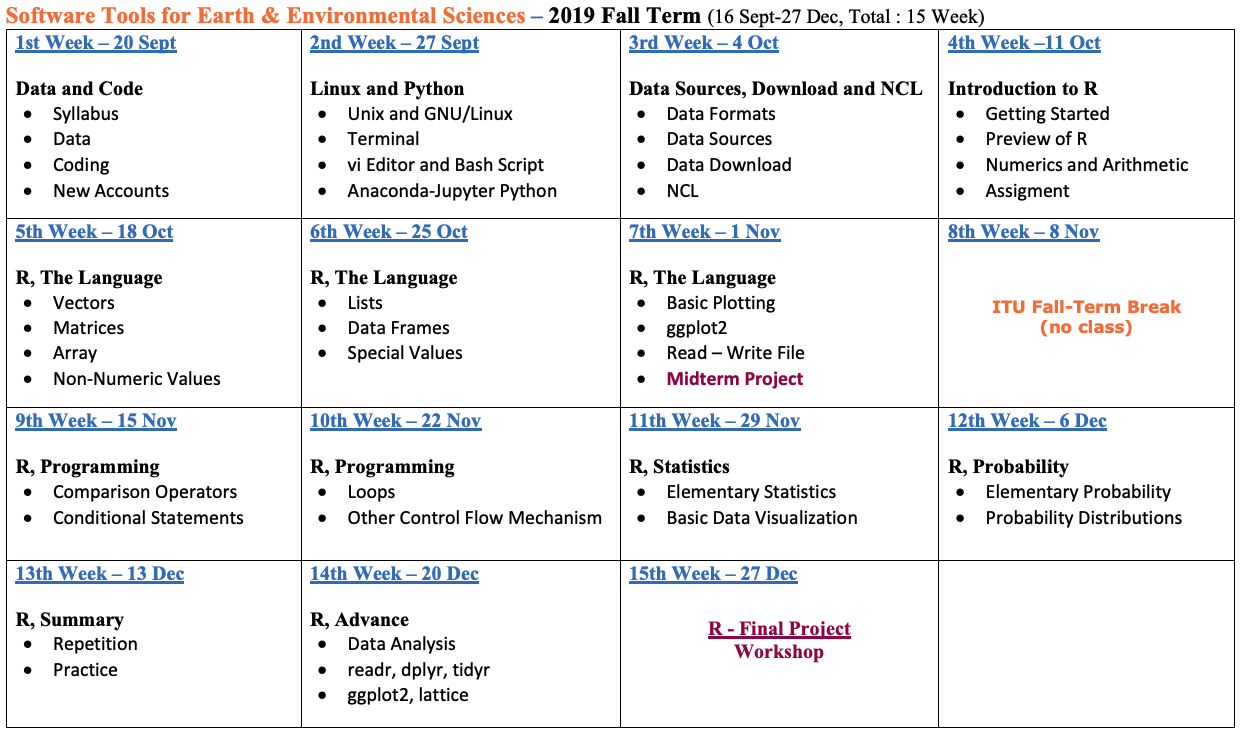
\includegraphics{syllabus.png} Extended Syllabus
\href{https://web.itu.edu.tr/~tokerem/Software_Tools_Syllabus.pdf}{PDF}

\end{block}

\begin{block}{\textbf{Book}}

\begin{figure}
\centering

\includegraphics{The_Book_of_R.png}
\caption{}
\end{figure}

The Book of R -
\href{https://web.itu.edu.tr/~tokerem/The_Book_of_R.pdf}{PDF}

\end{block}

\begin{block}{\textbf{Last Week}}

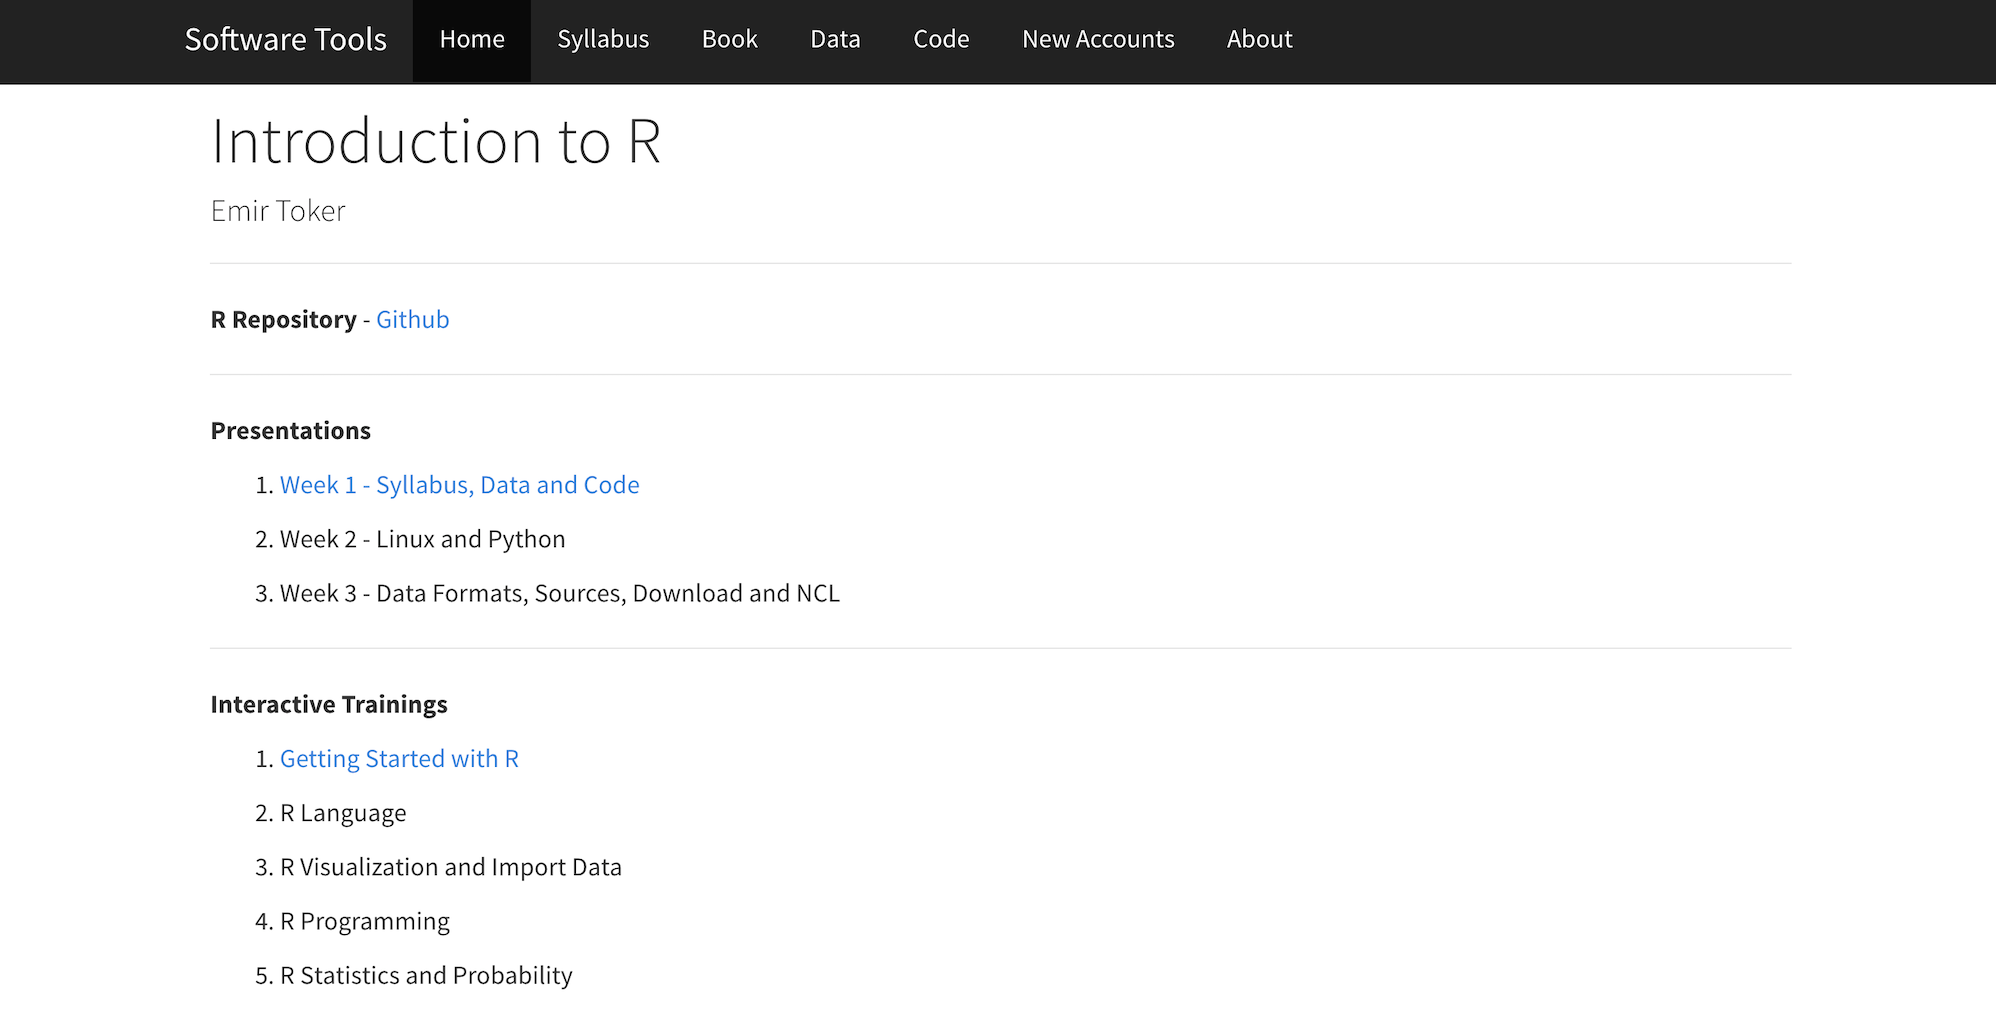
\includegraphics{last_week.png} Course Home Page
\href{https://emirtoker.github.io/Software_Tools_R_Github/index.html}{LINK}

Week 1 - Presentation
\href{http://rpubs.com/emirtoker/software_tools_week1}{LINK}

\end{block}

\end{frame}

\begin{frame}{\textbf{Unix}}

\begin{block}{\textbf{What is Unix?}}

\begin{itemize}
\tightlist
\item
  UNIX is a computer operating system.
\item
  It was first developed in 1969 at Bell Labs.
\item
  In 1972, the Unix code was rewritten with the new C programming
  language.
\end{itemize}

\begin{figure}
\centering
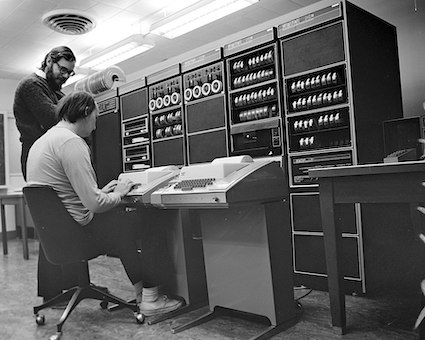
\includegraphics{unix_develop.jpg}
\caption{}
\end{figure}

(Dennis, Ken)

\end{block}

\end{frame}

\begin{frame}{\textbf{GNU}}

\begin{block}{\textbf{What is GNU?}}

\begin{itemize}
\tightlist
\item
  A wildebeest (or gnu) is an animal. Lives in Africa.
\item
  GNU is the name of a computer operating system.
\item
  The GNU project was started by Richard Stallman in 1983.
\item
  {\textbf{G}}NU's {\textbf{N}}ot {\textbf{U}}nix!
\item
  Fully free to modify, share and publish.
\end{itemize}


\includegraphics{gnu_logo.png} 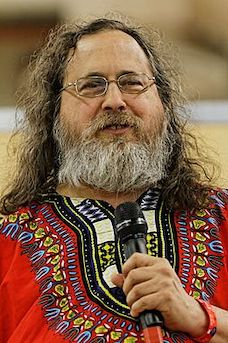
\includegraphics{Richard.jpg}

\end{block}

\end{frame}

\begin{frame}{\textbf{GNU/Linux}}

\begin{block}{\textbf{What is Linux (or GNU/Linux) ?}}

\begin{itemize}
\tightlist
\item
  Linux (or GNU/Linux) is a Unix-like operating system.
\item
  GNU did not have all the parts.
\item
  The kernel (GNU Hurd) is not yet completely built.
\item
  In 1991 Linus Torvalds began to work -\textgreater{} Linux kernel.
\end{itemize}

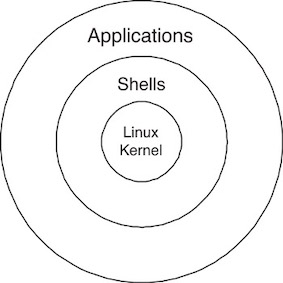
\includegraphics{kernel.jpg} 
\includegraphics{linux_logo.png}
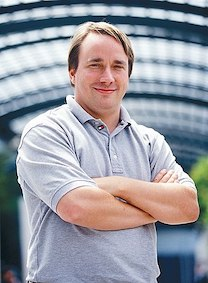
\includegraphics{linus.jpeg}

\end{block}

\begin{block}{\textbf{How is Unix different from Linux?}}

\begin{itemize}
\item
  Linux does not use code from UNIX.
\item
  The idea and names of commands are similar.
\end{itemize}

\begin{figure}
\centering

\includegraphics{unix_linux.png}
\caption{}
\end{figure}

\end{block}

\begin{block}{\textbf{GNU/Linux Distributions}}

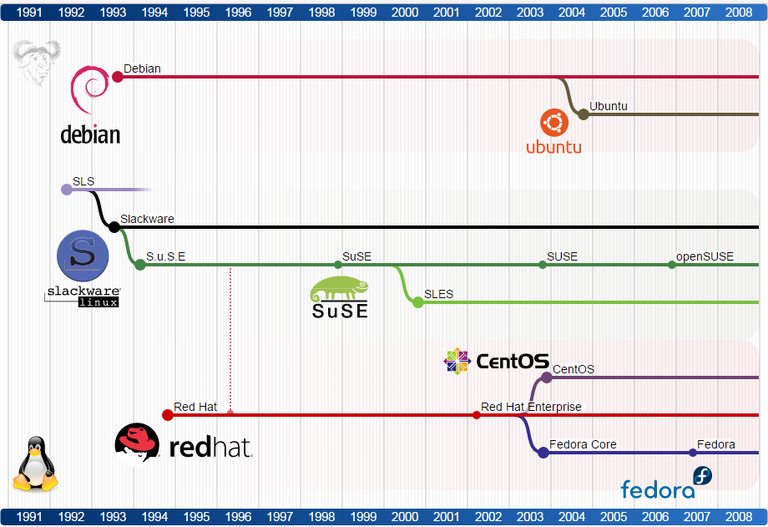
\includegraphics{linux_dist.png}
\href{https://upload.wikimedia.org/wikipedia/commons/1/1b/Linux_Distribution_Timeline.svg}{Linux\_Distribution\_Timeline}

\end{block}

\end{frame}

\begin{frame}{\textbf{Terminal}}

\begin{block}{\textbf{Terminal}}

A computer \textbf{terminal} is a \textbf{hardware device} that is used
for entering data into, and displaying or printing data from a computer
or a computing system.

\begin{figure}
\centering
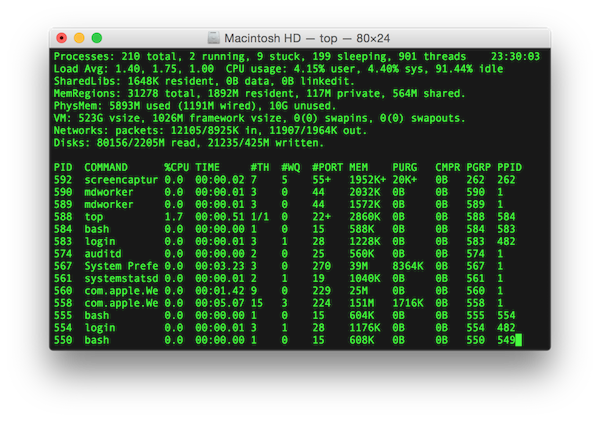
\includegraphics{terminal0.png}
\caption{}
\end{figure}

\end{block}

\begin{block}{\textbf{Terminal}}

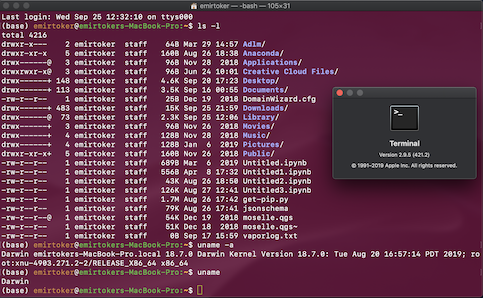
\includegraphics{terminal.png} 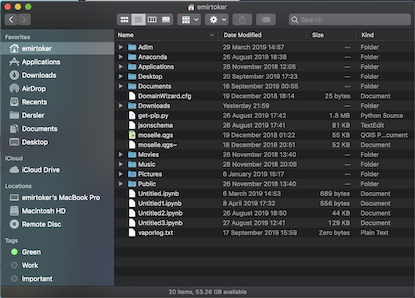
\includegraphics{terminal1.png}

\end{block}

\end{frame}

\begin{frame}{\textbf{Basic GNU/Linux Commands}}

\begin{block}{\textbf{Basic GNU/Linux Commands}}

\begin{itemize}
\item
  Frequently Used Terms
\item
  Directory Commands
\item
  File Commands
\item
  Special Commands
\item
  vi Editor, Print Commands and Symbols
\end{itemize}

\end{block}

\end{frame}

\begin{frame}[fragile]{\textbf{Frequently Used Terms}}

\begin{block}{\textbf{Frequently Used Terms}}

\begin{itemize}
\tightlist
\item
  File and Folder
\item
  Directory

  \begin{itemize}
  \tightlist
  \item
    Parent Directory
  \item
    Working Directory
  \end{itemize}
\item
  User
\item
  Root or Root Directory
\item
  Environments
\item
  Backup
\item
  Command, Command Line, Console
\item
  Warning, Error, Permission Denied
\item
  Segmentation Fault
\end{itemize}

\end{block}

\begin{block}{\textbf{Frequently Used Terms}}

\begin{itemize}
\tightlist
\item
  File and Folder
\item
  Directory Path, Parent and Working Directory
\end{itemize}

\begin{figure}
\centering
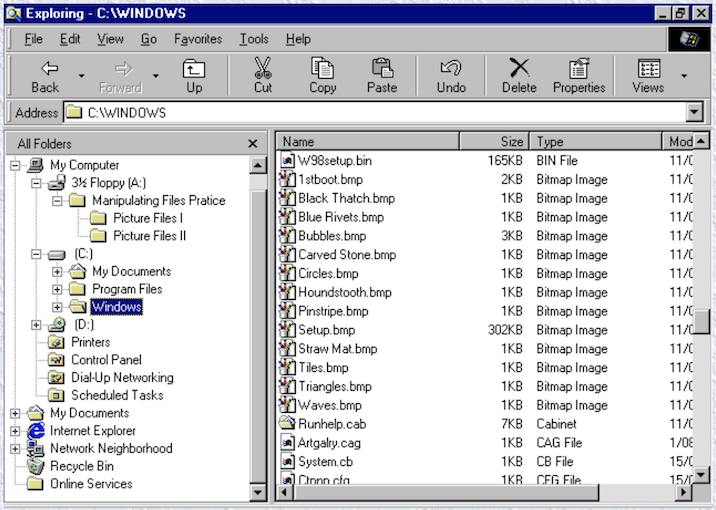
\includegraphics{filer_folder.png}
\caption{}
\end{figure}

\end{block}

\begin{block}{\textbf{Frequently Used Terms}}

User, Root and Home Directory

\begin{Shaded}
\begin{Highlighting}[]
\FunctionTok{whoami}
\end{Highlighting}
\end{Shaded}

\begin{verbatim}
## emirtoker
\end{verbatim}

Root directory symbol; ``\textbf{\texttt{/}}''. Home directory symbol;
``\textbf{\texttt{\textasciitilde{}}}''.

\begin{figure}
\centering
\includegraphics{root_fig.gif}
\caption{}
\end{figure}

\end{block}

\begin{block}{\textbf{Frequently Used Terms}}

Environments and Backup

\begin{verbatim}
printenv  
\end{verbatim}

\begin{figure}
\centering
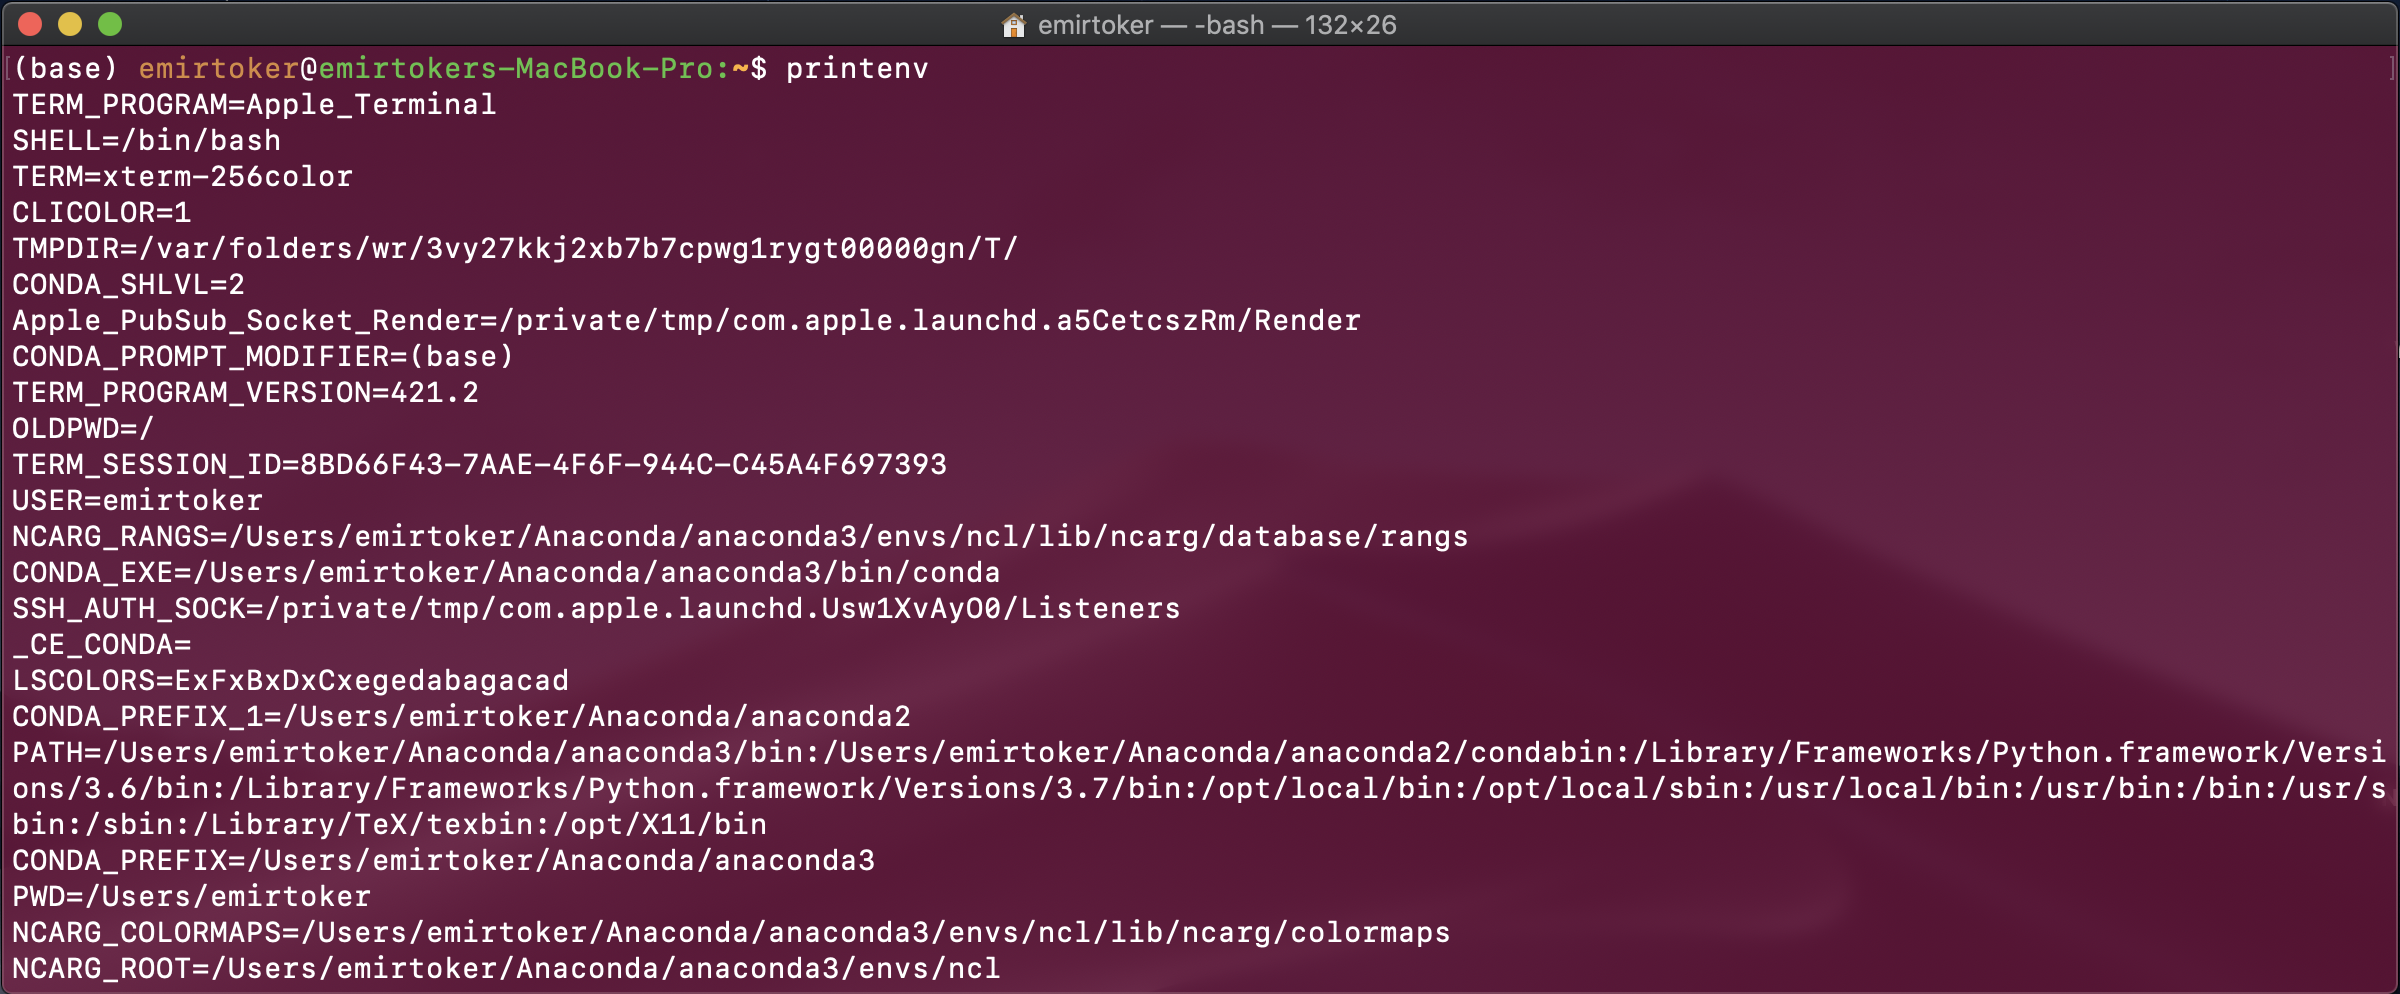
\includegraphics{printenv.png}
\caption{}
\end{figure}

\end{block}

\begin{block}{\textbf{Frequently Used Terms}}

Command Line, Command

\begin{figure}
\centering
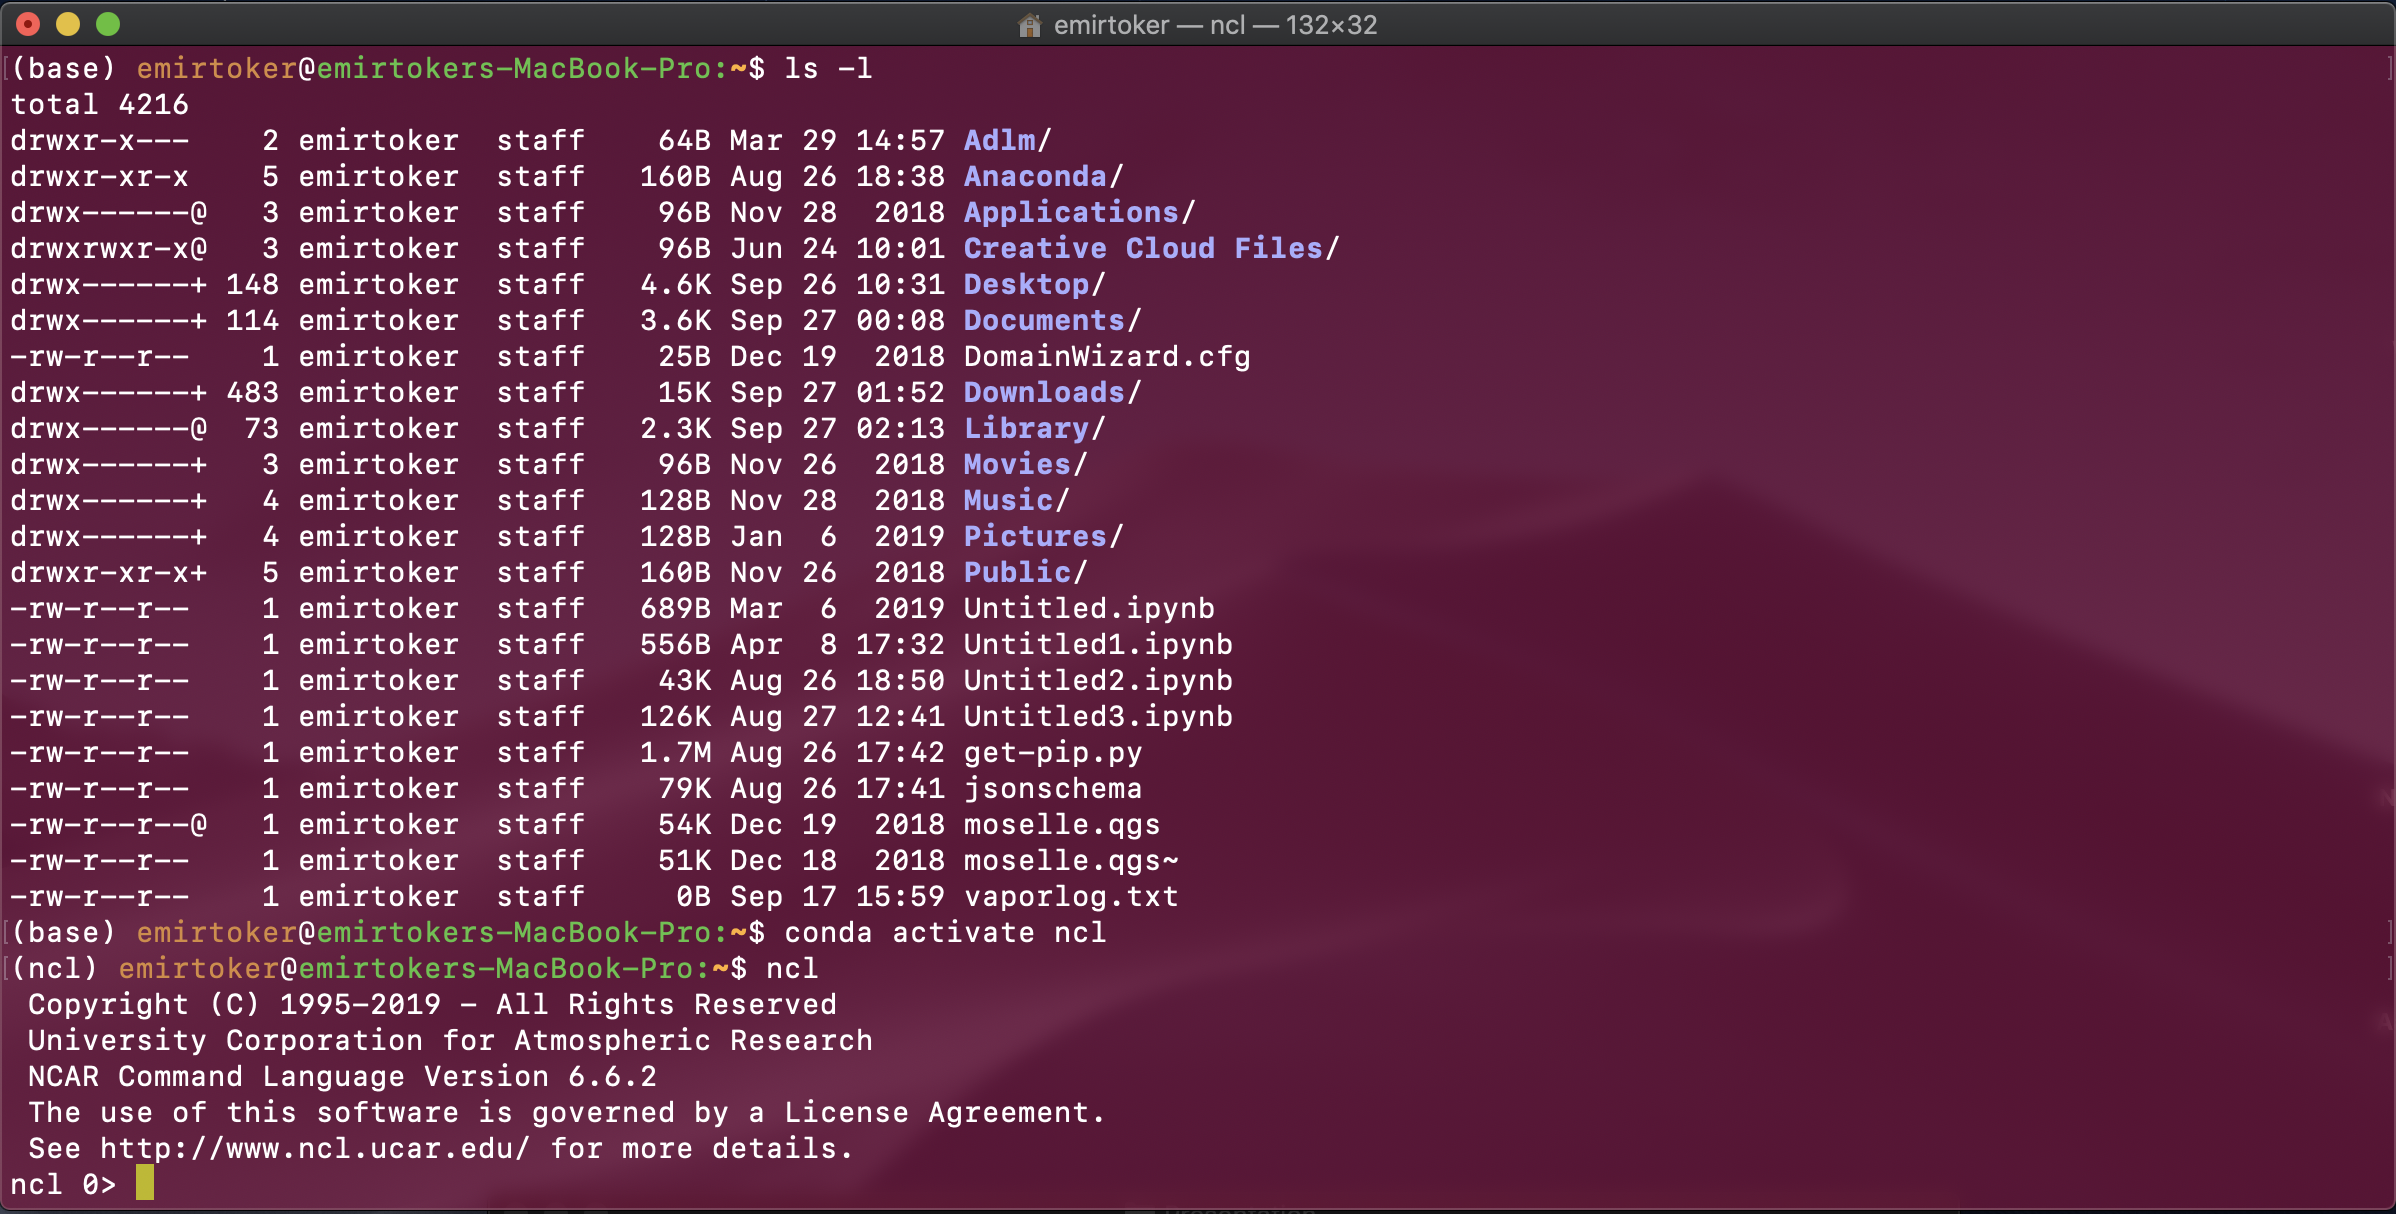
\includegraphics{command_line.png}
\caption{}
\end{figure}

\end{block}

\begin{block}{\textbf{Frequently Used Terms}}

Warning, Error, Permission Denied, Segmentation Fault

\begin{figure}
\centering
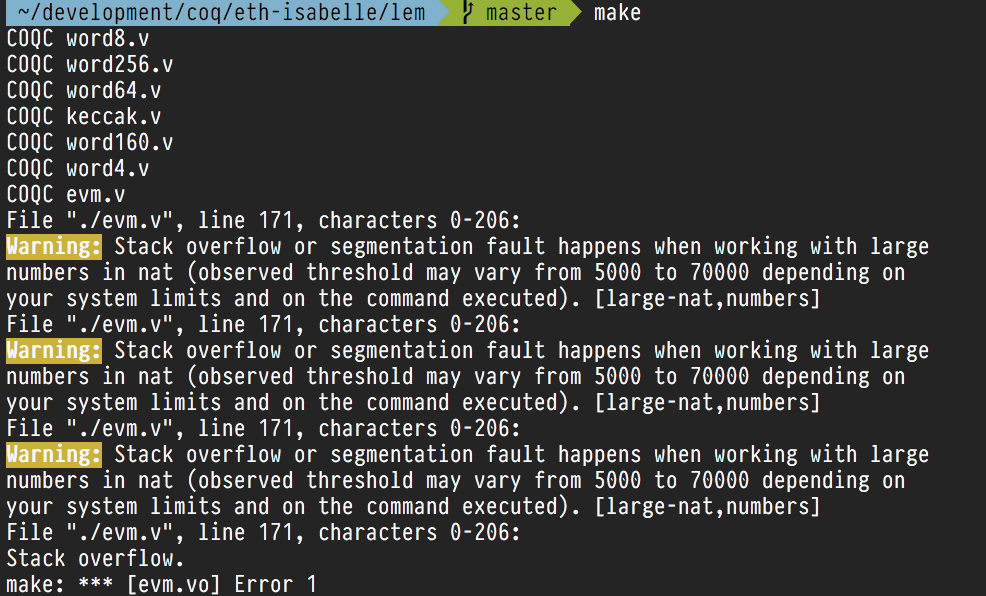
\includegraphics{warning.png}
\caption{}
\end{figure}

\end{block}

\end{frame}

\begin{frame}[fragile]{\textbf{Directory Commands}}

\begin{block}{\textbf{Directory Commands}}

\begin{itemize}
\item
  {\textbf{pwd}} \emph{(\textbf{P}rint \textbf{W}orking
  \textbf{D}irectory)}
\item
  {\textbf{ls}} \emph{(\textbf{L}ist \textbf{D}irectories)}
\item
  {\textbf{cd}} \emph{(\textbf{C}hange \textbf{D}irectory)}
\item
  {\textbf{mkdir}} \emph{(\textbf{M}ake \textbf{D}irectory)}
\end{itemize}

\end{block}

\begin{block}{\textbf{Directory Commands - {\textbf{pwd}}}}

\emph{(\textbf{P}rint \textbf{W}orking \textbf{D}irectory)}

\begin{Shaded}
\begin{Highlighting}[]
\BuiltInTok{pwd}
\end{Highlighting}
\end{Shaded}

\begin{verbatim}
## /Users/emirtoker/Desktop/Dersler/Memurluk/Software_Tools_for_Earth_&_Environmental_Science/Software_Tools_R_Github/Presentation
\end{verbatim}

\begin{figure}
\centering
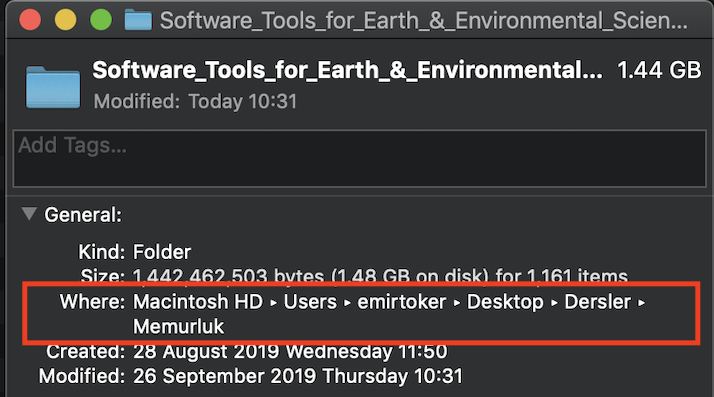
\includegraphics{pwd_mac1.png}
\caption{}
\end{figure}

\end{block}

\begin{block}{\textbf{Directory Commands - {\textbf{ls}}}}

\emph{(\textbf{L}ist \textbf{D}irectories)}

\begin{Shaded}
\begin{Highlighting}[]
\FunctionTok{ls}
\end{Highlighting}
\end{Shaded}

\begin{verbatim}
## Presentation.Rproj
## Presentation_Week1_-_Data_and_Code.Rmd
## Presentation_Week1_-_Data_and_Code.html
## Presentation_Week2_-_Linux_and_Python.Rmd
## Presentation_Week2_-_Linux_and_Python.html
## Presentation_Week2_-_Linux_and_Python.pdf
## Richard.jpg
## Software_Tools_for_Earth_and_Environmental_Science_Syllabus.png
## The_Book_of_R.png
## Week1_rpubs.Rmd
## Week1_rpubs.html
## ai.png
## algorithm.png
## alma.jpg
## anaconda.png
## analysis.png
## apache_point.jpg
## arcgis.png
## big_data1.png
## book_flow.png
## cd1.png
## cd2.png
## clear.png
## code.png
## command_line.png
## conda.png
## course_github.png
## coursera.png
## cp.png
## cp1.png
## cygwin.png
## data_analytics.png
## data_assim.jpeg
## data_mining.svg
## datacamp.png
## datascience.png
## datashape.jpg
## datum.png
## deep.jpg
## download.png
## dropbox.png
## earthdata.png
## eda.png
## edx.png
## exit.png
## extended_syllabus.png
## extended_syllabus1.png
## filer_folder.png
## filezilla.png
## find.png
## generate.png
## github.png
## gnu_logo.png
## help.png
## history.png
## iot.png
## jupyter.png
## jupyter_notebook.png
## kernel.jpg
## khanacademy.png
## languages.png
## last_week.png
## linus.jpeg
## linux_dist.png
## linux_logo.png
## machine.jpg
## mendeley.png
## metadata0.png
## metadata1.png
## meted.png
## mining.jpg
## mining1.jpg
## mkdir1.png
## mkdir2.png
## model.png
## mv.png
## my_profile
## mynewfile.png
## nc.png
## ncl.png
## orcid.png
## os.png
## overleaf.png
## panoply.png
## printenv.png
## pwd_mac.png
## pwd_mac1.png
## pwd_win.png
## python.jpg
## python_term.png
## qgis.png
## researchgate.png
## rm.png
## root.png
## root_fig.gif
## rsconnect
## rstudio.png
## simulation.jpg
## stackoverflow.png
## sublimetext.png
## syllabus.png
## terminal.png
## terminal0.png
## terminal1.png
## touch.png
## udemy.png
## unix_develop.jpg
## unix_linux.png
## vi_0.png
## vi_1.png
## vi_2.png
## vi_3.png
## visual.jpg
## warning.png
## week2_sil.Rmd
## week2_sil.pdf
## week2_sil_files
## wetransfer.png
## wget.jpg
## what_data.svg
## win_folder.png
## wolfram-alpha.png
## zenodo-doi.png
\end{verbatim}

\end{block}

\begin{block}{\textbf{Directory Commands - pwd and ls}}

\begin{figure}
\centering
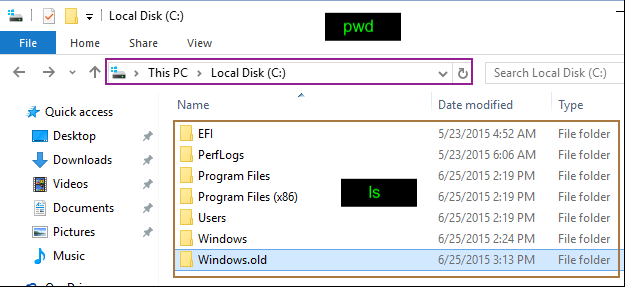
\includegraphics{win_folder.png}
\caption{}
\end{figure}

\end{block}

\begin{block}{\textbf{Directory Commands - {\textbf{cd}}}}

\emph{(\textbf{C}hange \textbf{D}irectory)}

\begin{verbatim}
cd Presentation/
\end{verbatim}

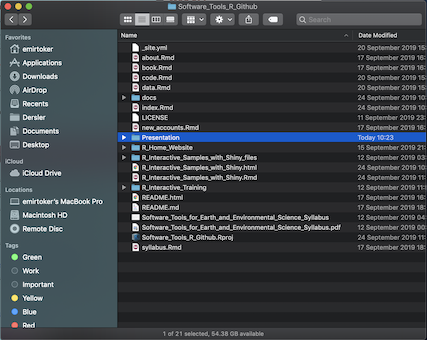
\includegraphics{cd1.png} 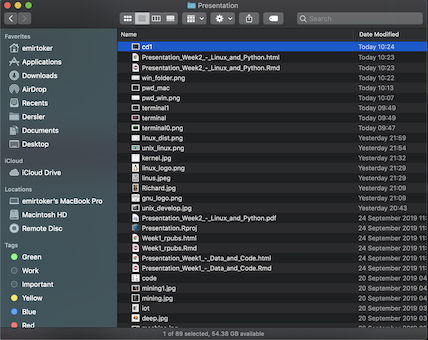
\includegraphics{cd2.png}

\end{block}

\begin{block}{\textbf{Directory Commands - {\textbf{mkdir}}}}

\emph{(\textbf{M}ake \textbf{D}irectory)}

\begin{verbatim}
mkdir <new_folder_name>
\end{verbatim}

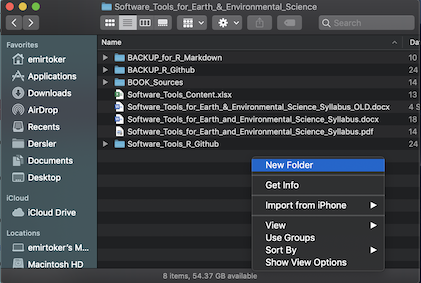
\includegraphics{mkdir1.png} 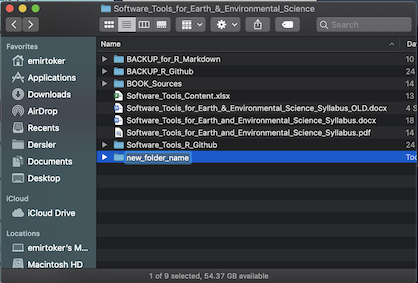
\includegraphics{mkdir2.png}

\end{block}

\end{frame}

\begin{frame}[fragile]{\textbf{File Commands}}

\begin{block}{\textbf{File Commands}}

\begin{itemize}
\item
  {\textbf{touch}}
\item
  {\textbf{cat}} \emph{(Concatenate)}
\item
  {\textbf{rm}} \emph{(Remove)}
\item
  {\textbf{cp}} \emph{(Copy)}
\item
  {\textbf{mv}} \emph{(Move)}
\end{itemize}

\end{block}

\begin{block}{\textbf{File Commands - {\textbf{touch}}}}

\begin{verbatim}
touch <my_new_file>
\end{verbatim}

\begin{figure}
\centering
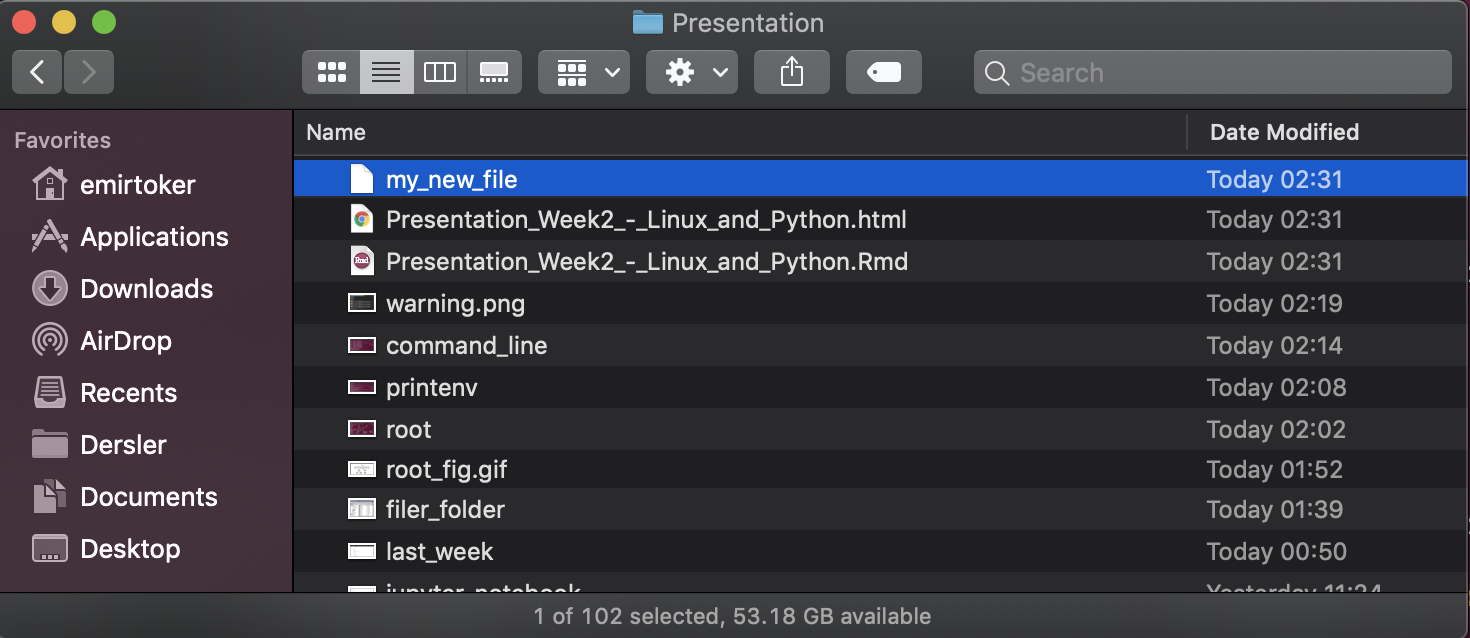
\includegraphics{touch.png}
\caption{}
\end{figure}

\end{block}

\begin{block}{\textbf{File Commands - {\textbf{cat}}}}

\emph{(Con\textbf{cat}enate)}

\begin{verbatim}
cat my_new_file
\end{verbatim}

\begin{verbatim}
This is my new file. Hi!
\end{verbatim}

\begin{figure}
\centering
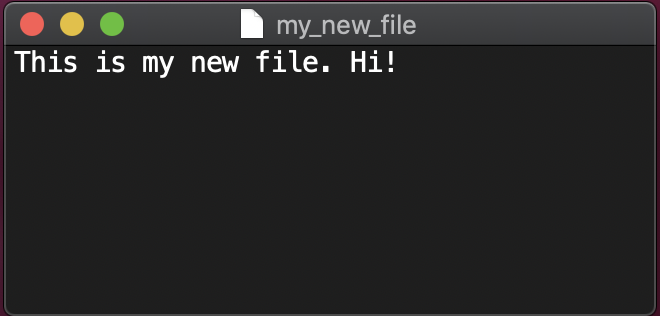
\includegraphics{mynewfile.png}
\caption{}
\end{figure}

\end{block}

\begin{block}{\textbf{File Commands - {\textbf{cp}}}}

\emph{(\textbf{C}o\textbf{p}y)}

\begin{verbatim}
cp my_new_file my_new_file2
\end{verbatim}

\begin{figure}
\centering
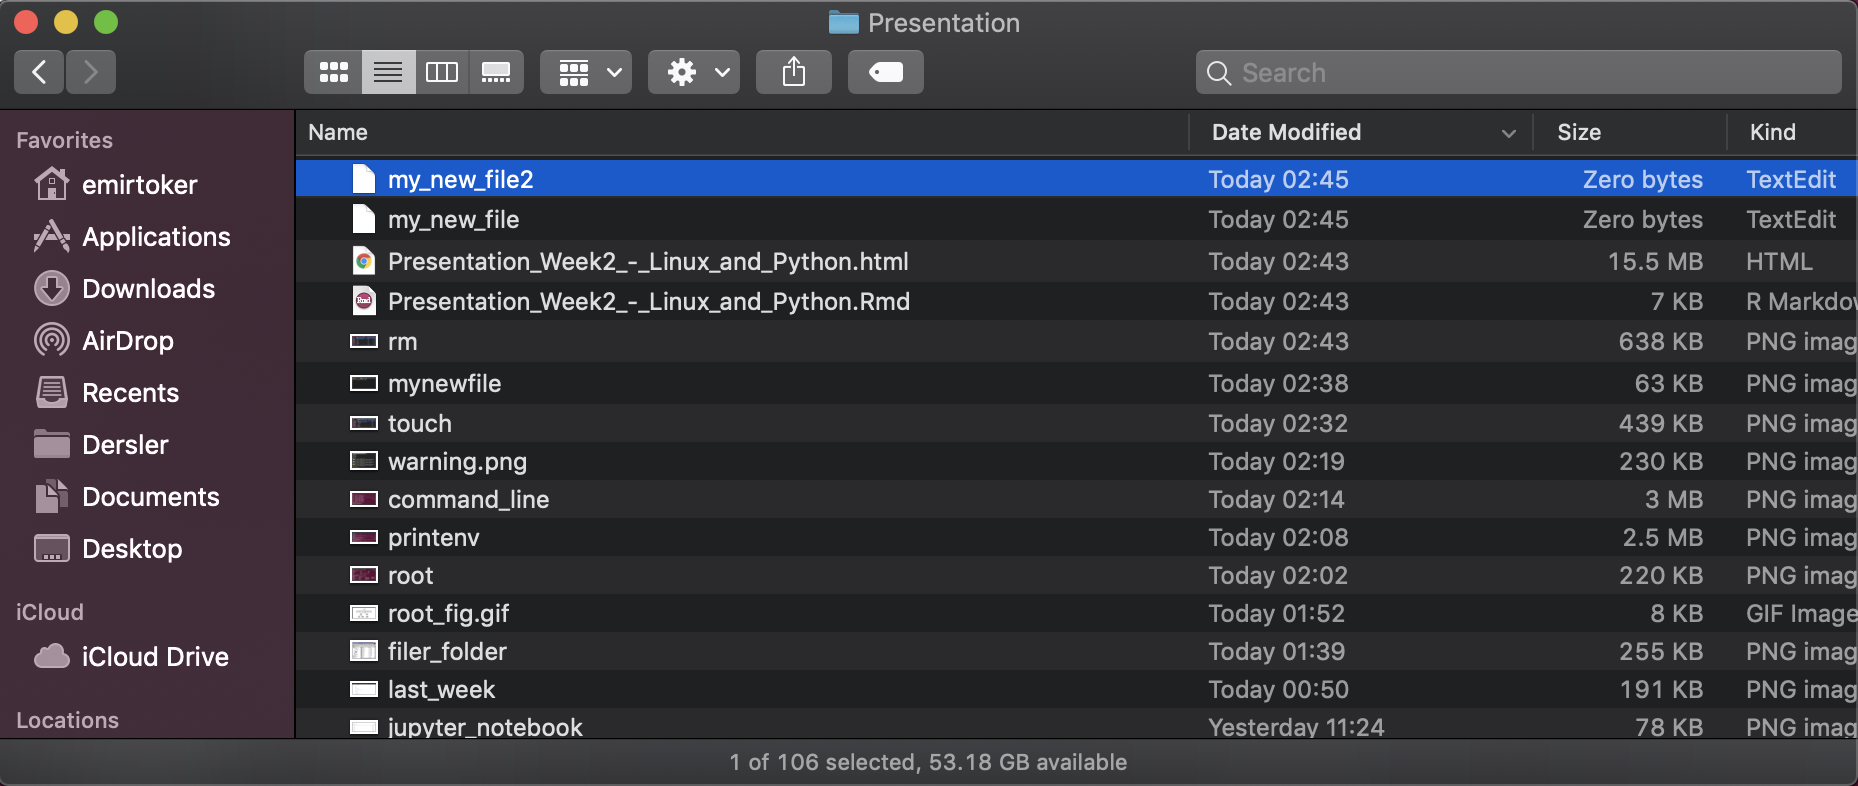
\includegraphics{cp.png}
\caption{}
\end{figure}

\end{block}

\begin{block}{\textbf{File Commands - {\textbf{mv}}}}

\emph{(\textbf{M}o\textbf{v}e)}

\begin{verbatim}
mv my_new_file2 my_new_file3
\end{verbatim}

\begin{figure}
\centering
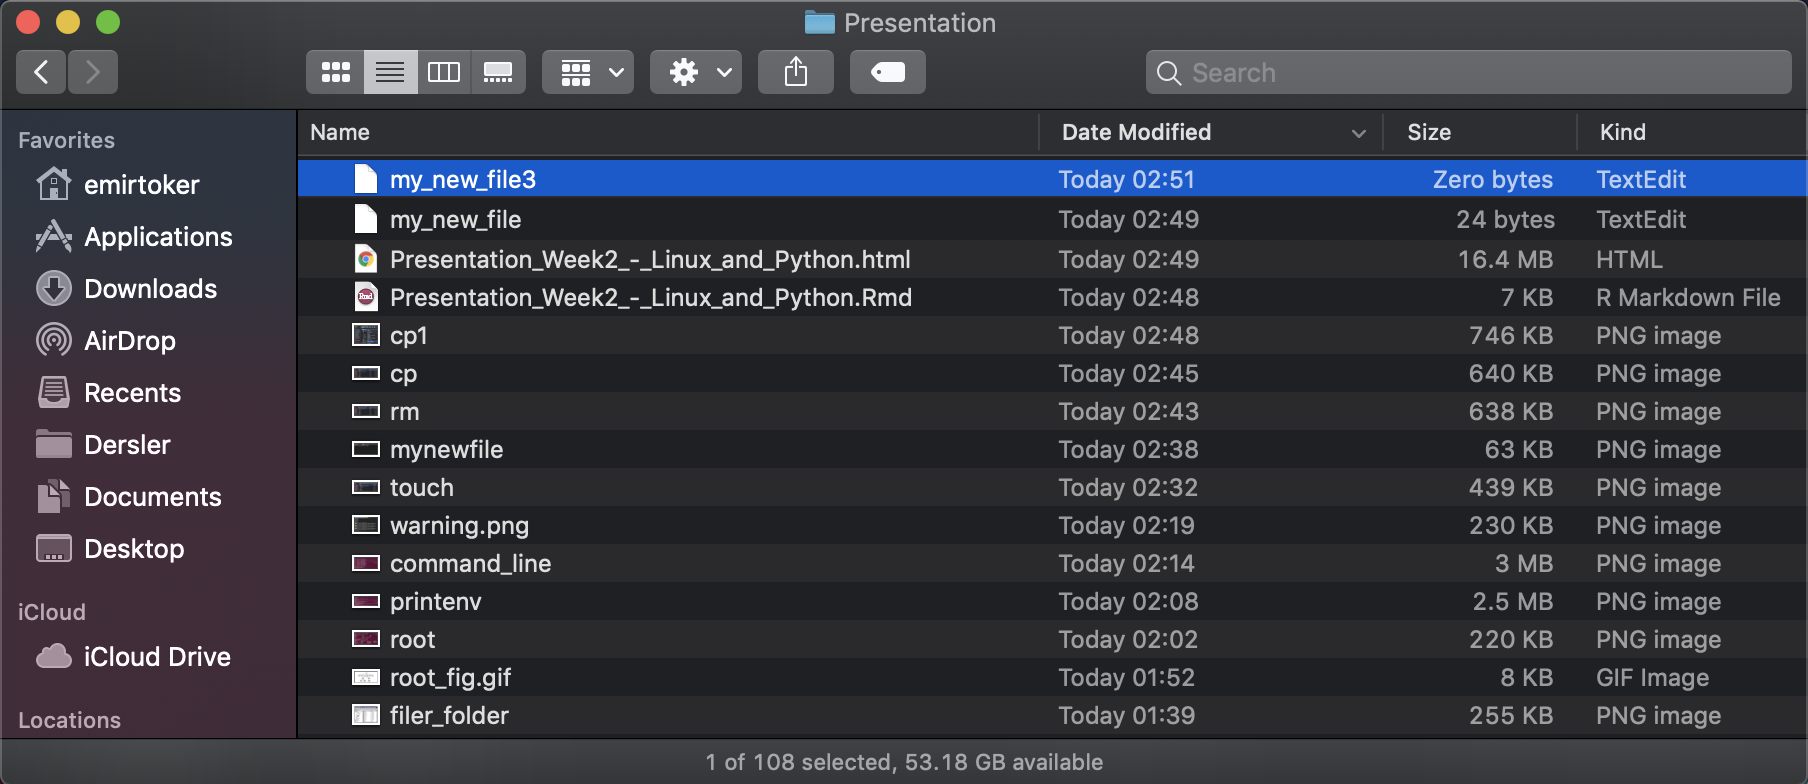
\includegraphics{mv.png}
\caption{}
\end{figure}

\end{block}

\begin{block}{\textbf{File Commands - {\textbf{rm}}}}

\emph{(\textbf{R}e\textbf{m}ove)}

\begin{verbatim}
rm my_new_file my_new_file3
\end{verbatim}

\begin{figure}
\centering
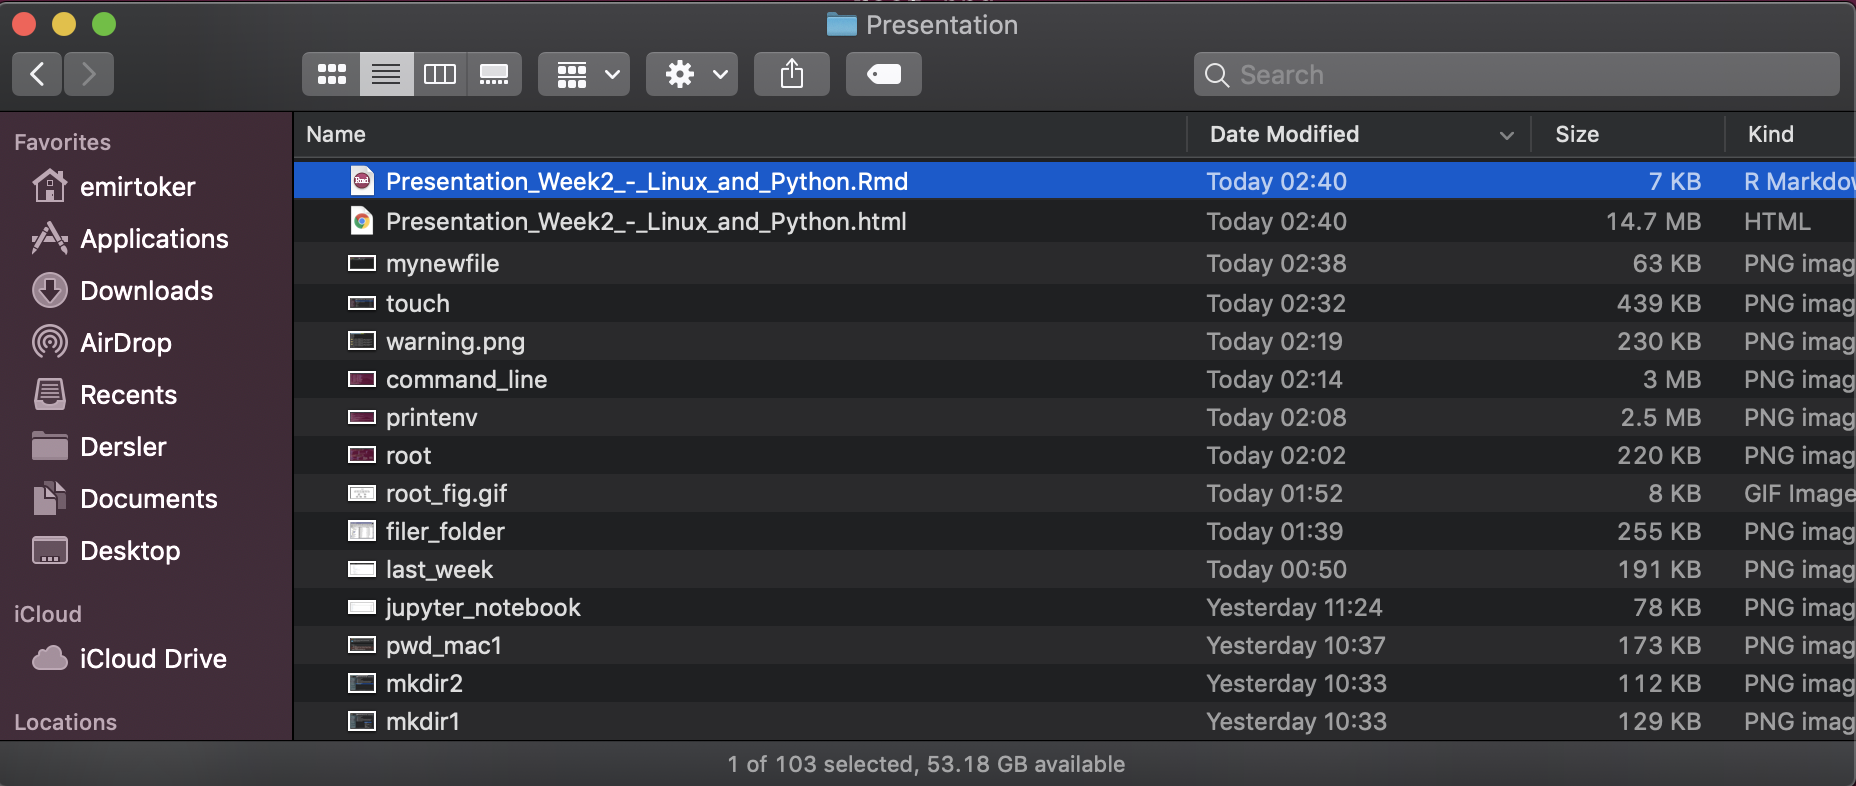
\includegraphics{rm.png}
\caption{}
\end{figure}

\end{block}

\end{frame}

\begin{frame}[fragile]{\textbf{Special Commands}}

\begin{block}{\textbf{Special Commands}}

\begin{itemize}
\item
  \textbf{{\textbf{find}}}
\item
  \textbf{{\textbf{help}}}
\item
  \textbf{{\textbf{history}}}
\item
  \textbf{{\textbf{clear}}}
\item
  \textbf{{\textbf{date}}} and \textbf{{\textbf{cal}}}
\item
  \textbf{{\textbf{exit}}}
\end{itemize}

\end{block}

\begin{block}{\textbf{Special Commands - {\textbf{find}}}}

\begin{verbatim}
find -name <name_of_file>
\end{verbatim}

\begin{figure}
\centering
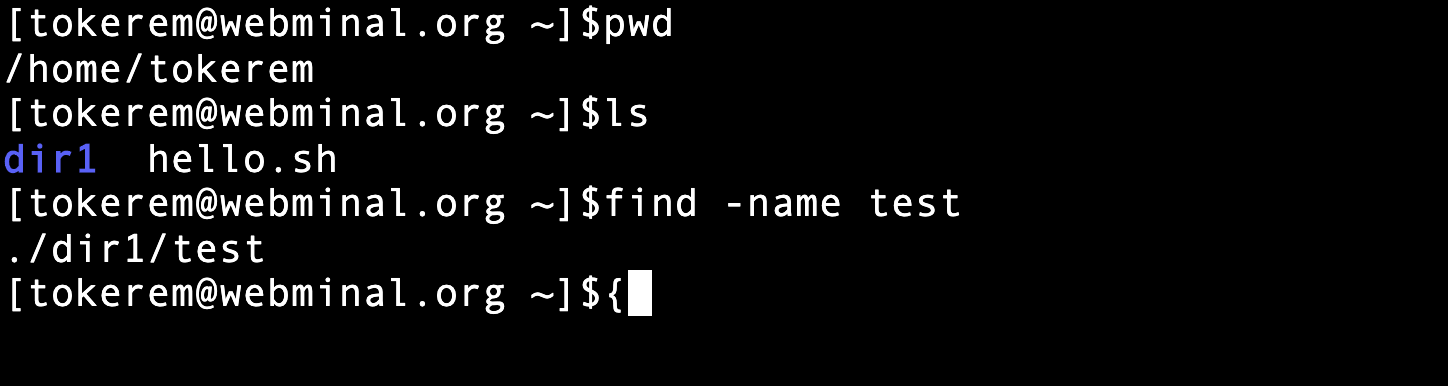
\includegraphics{find.png}
\caption{}
\end{figure}

\end{block}

\begin{block}{\textbf{Special Commands - {\textbf{help}}}}

\begin{verbatim}
find --help
\end{verbatim}

\begin{figure}
\centering
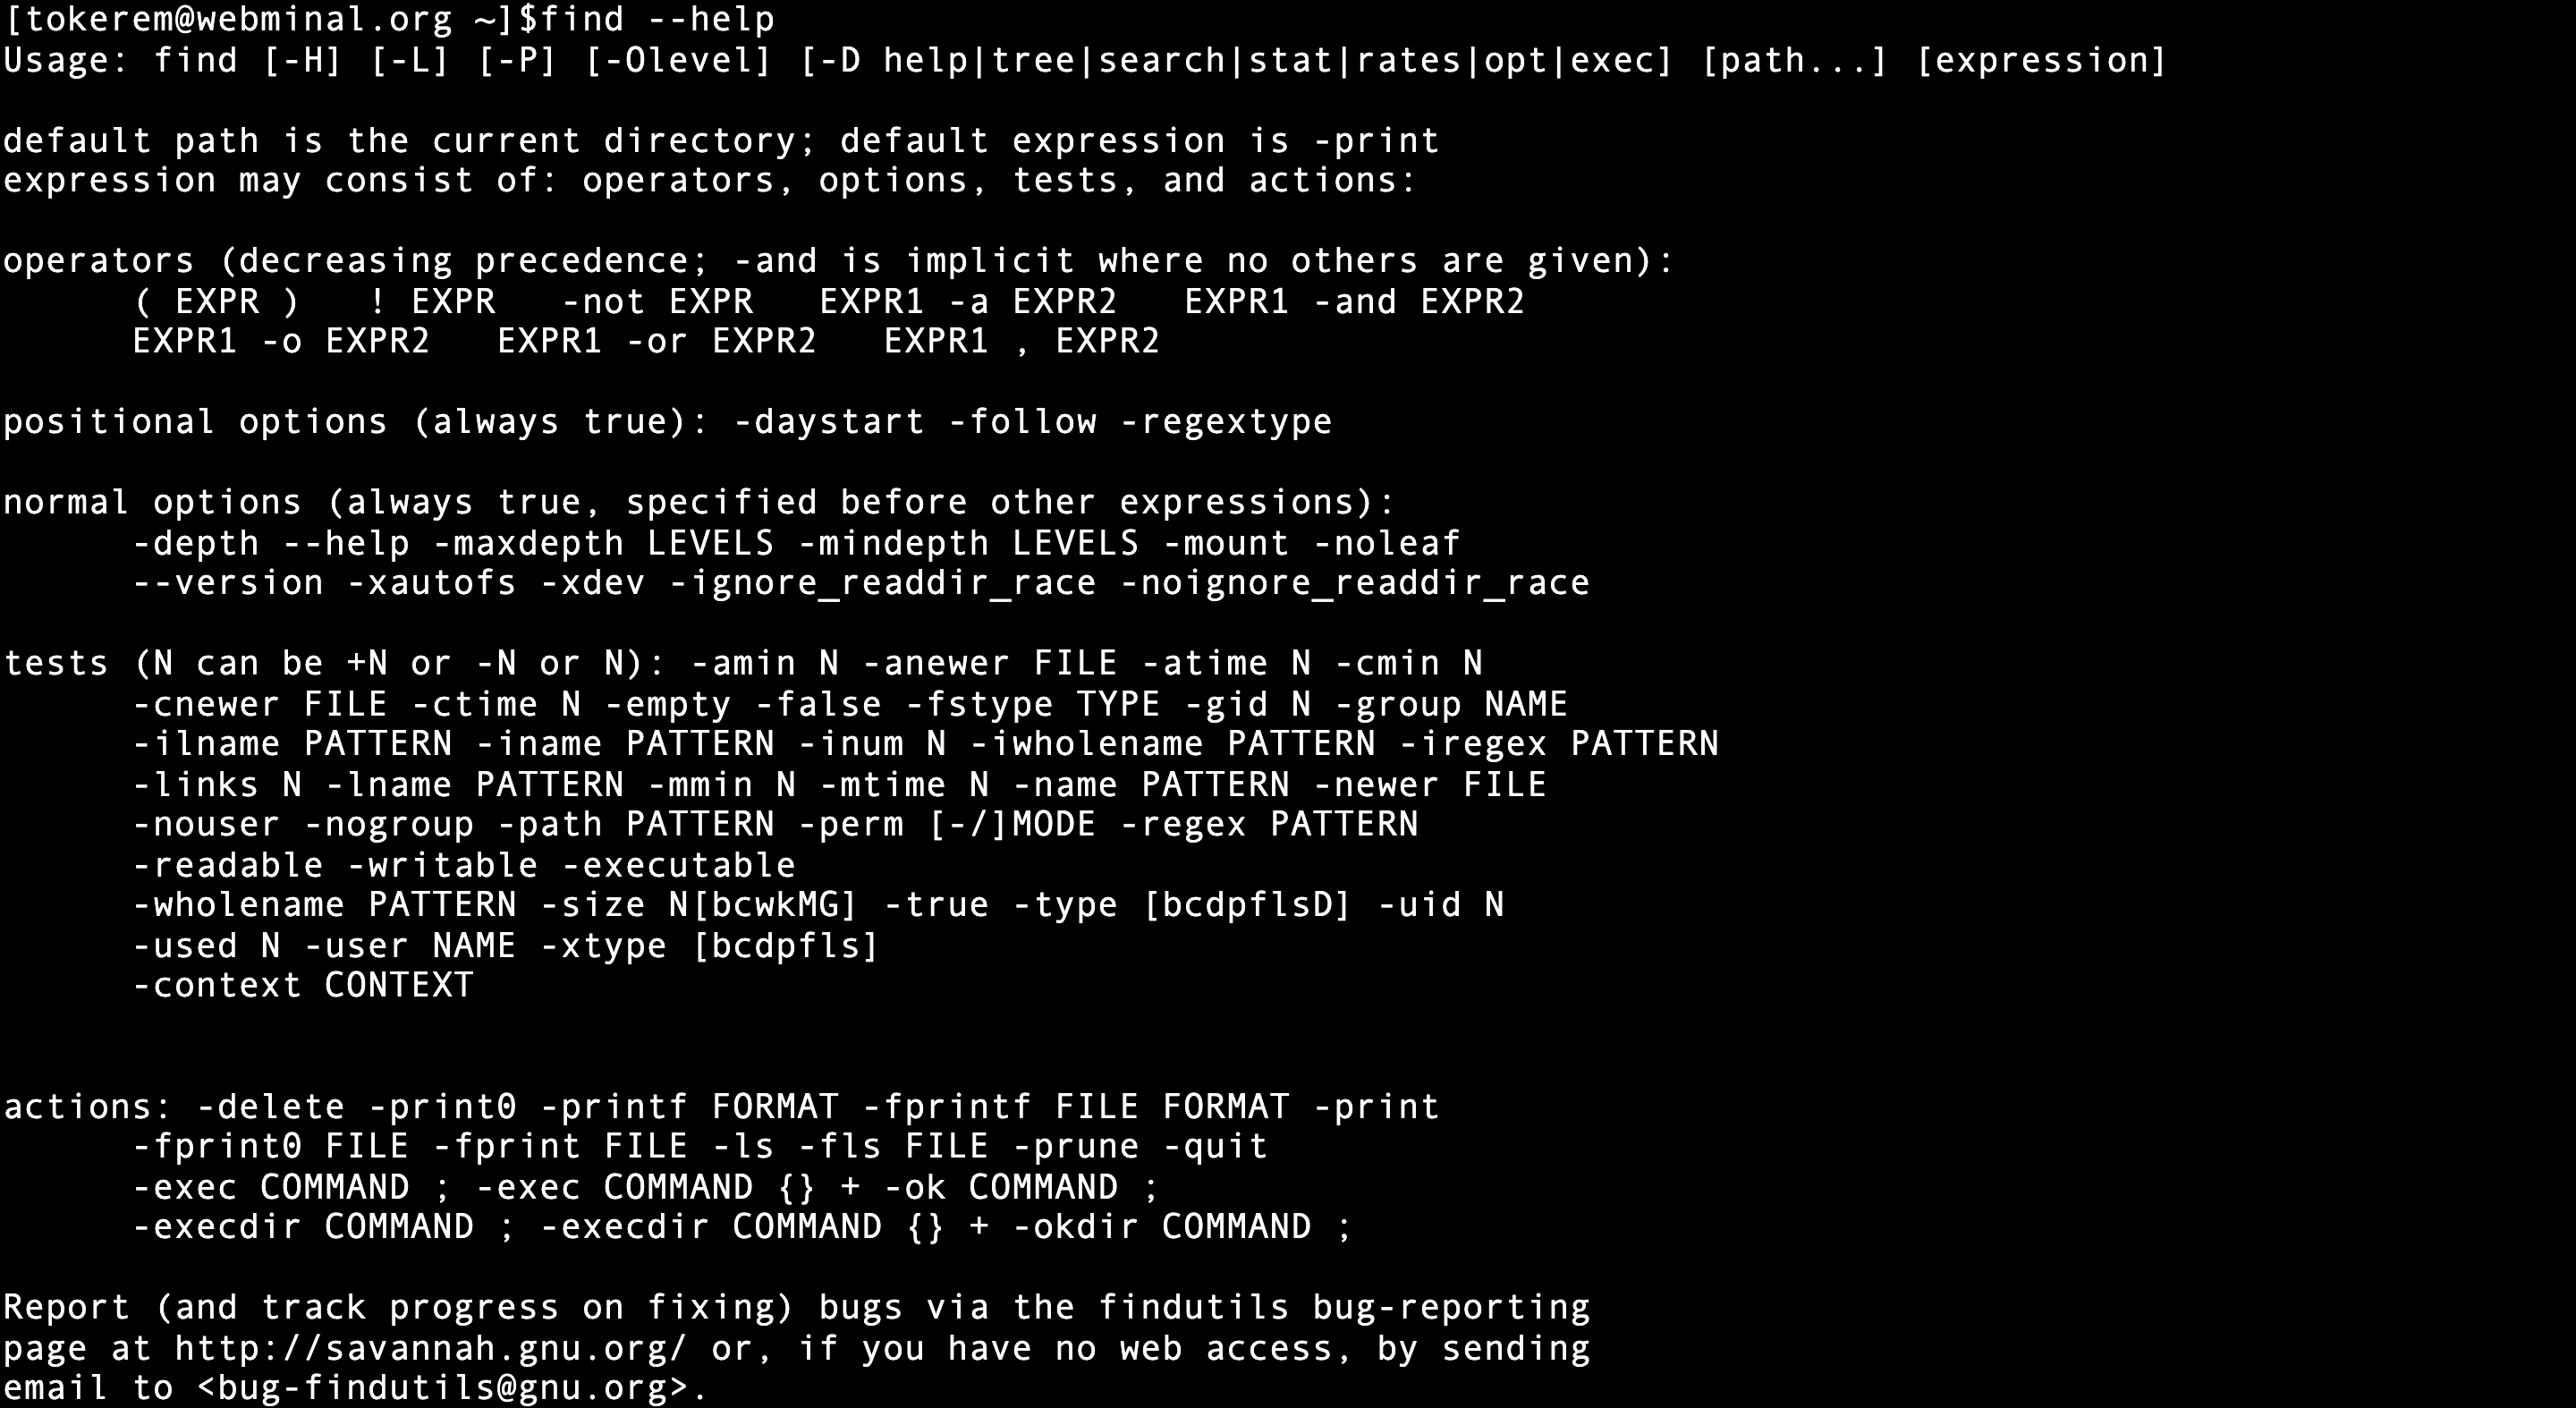
\includegraphics{help.png}
\caption{}
\end{figure}

\end{block}

\begin{block}{\textbf{Special Commands - {\textbf{history}}}}

\begin{verbatim}
history
\end{verbatim}

\begin{figure}
\centering
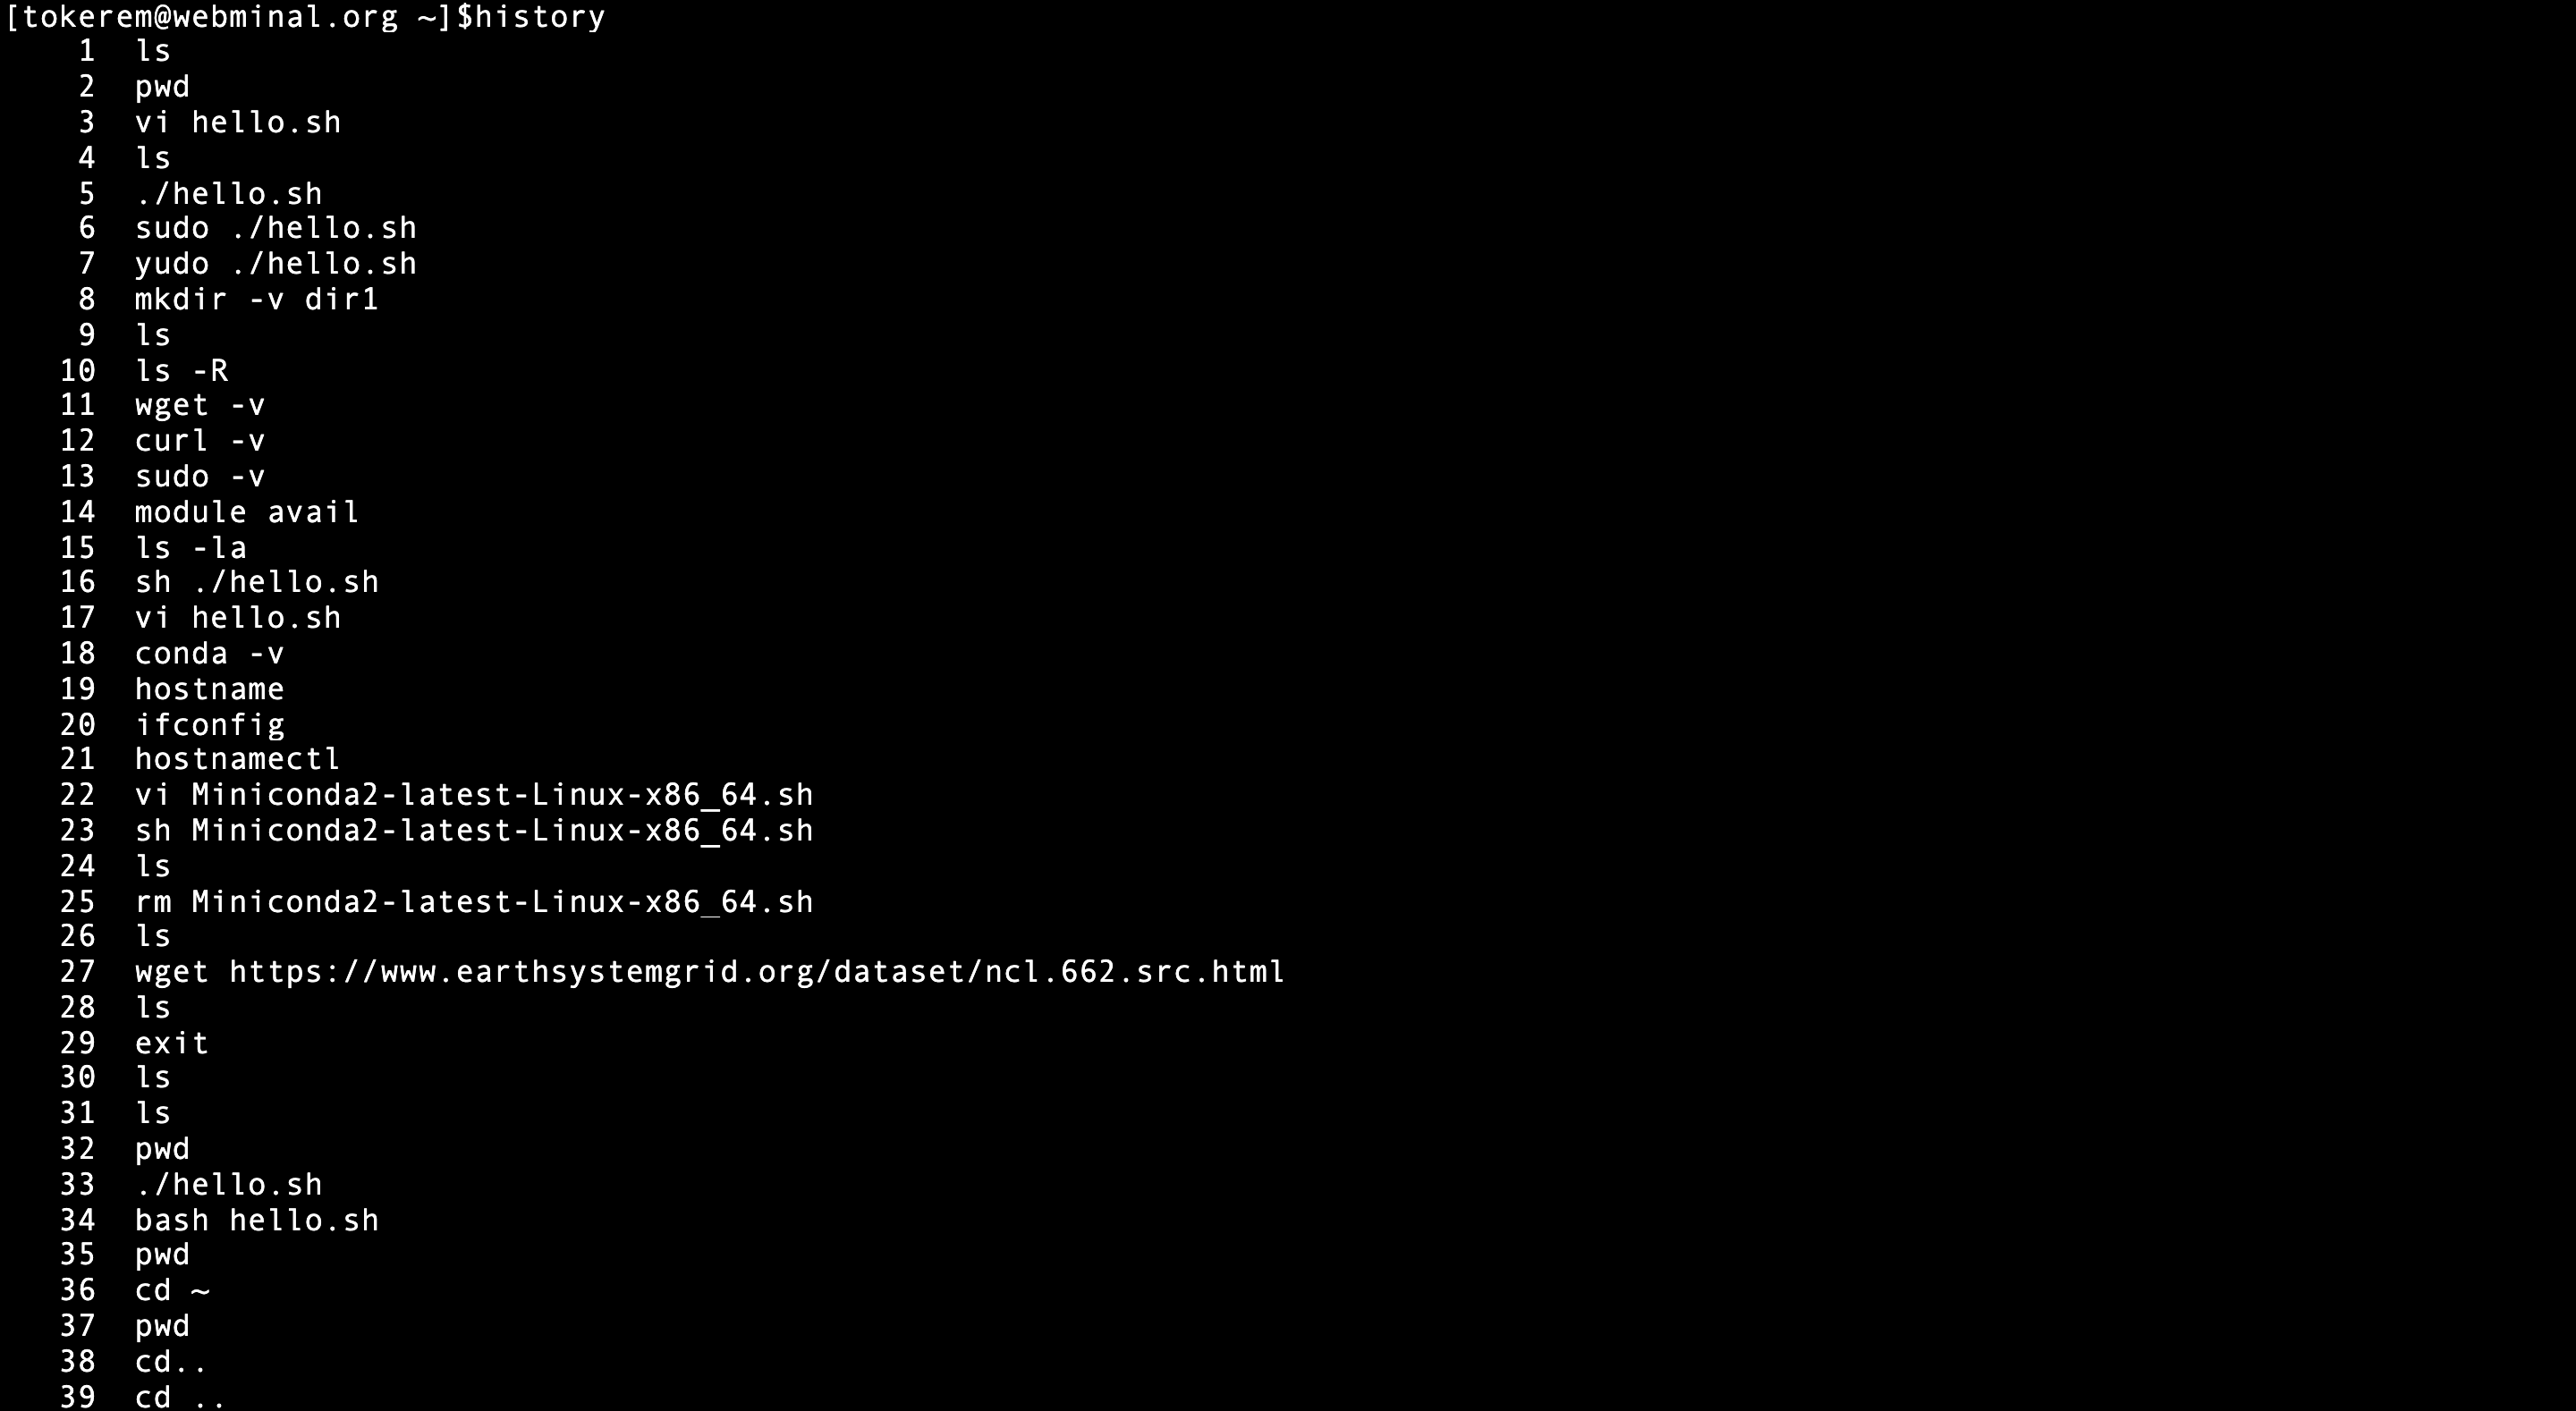
\includegraphics{history.png}
\caption{}
\end{figure}

\end{block}

\begin{block}{\textbf{Special Commands - {\textbf{clear}}}}

\begin{verbatim}
clear
\end{verbatim}

\begin{figure}
\centering

\includegraphics{clear.png}
\caption{}
\end{figure}

\end{block}

\begin{block}{\textbf{Special Commands - {\textbf{date}} and
{\textbf{cal}}}}

\begin{Shaded}
\begin{Highlighting}[]
\FunctionTok{date}
\end{Highlighting}
\end{Shaded}

\begin{verbatim}
## Mon Sep 30 15:59:49 +03 2019
\end{verbatim}

\begin{Shaded}
\begin{Highlighting}[]
\FunctionTok{cal}
\end{Highlighting}
\end{Shaded}

\begin{verbatim}
##    September 2019     
## Su Mo Tu We Th Fr Sa  
##  1  2  3  4  5  6  7  
##  8  9 10 11 12 13 14  
## 15 16 17 18 19 20 21  
## 22 23 24 25 26 27 28  
## 29 _3_0                 
## 
\end{verbatim}

\end{block}

\begin{block}{\textbf{Special Commands - {\textbf{exit}}}}

\begin{verbatim}
exit
\end{verbatim}

\begin{figure}
\centering
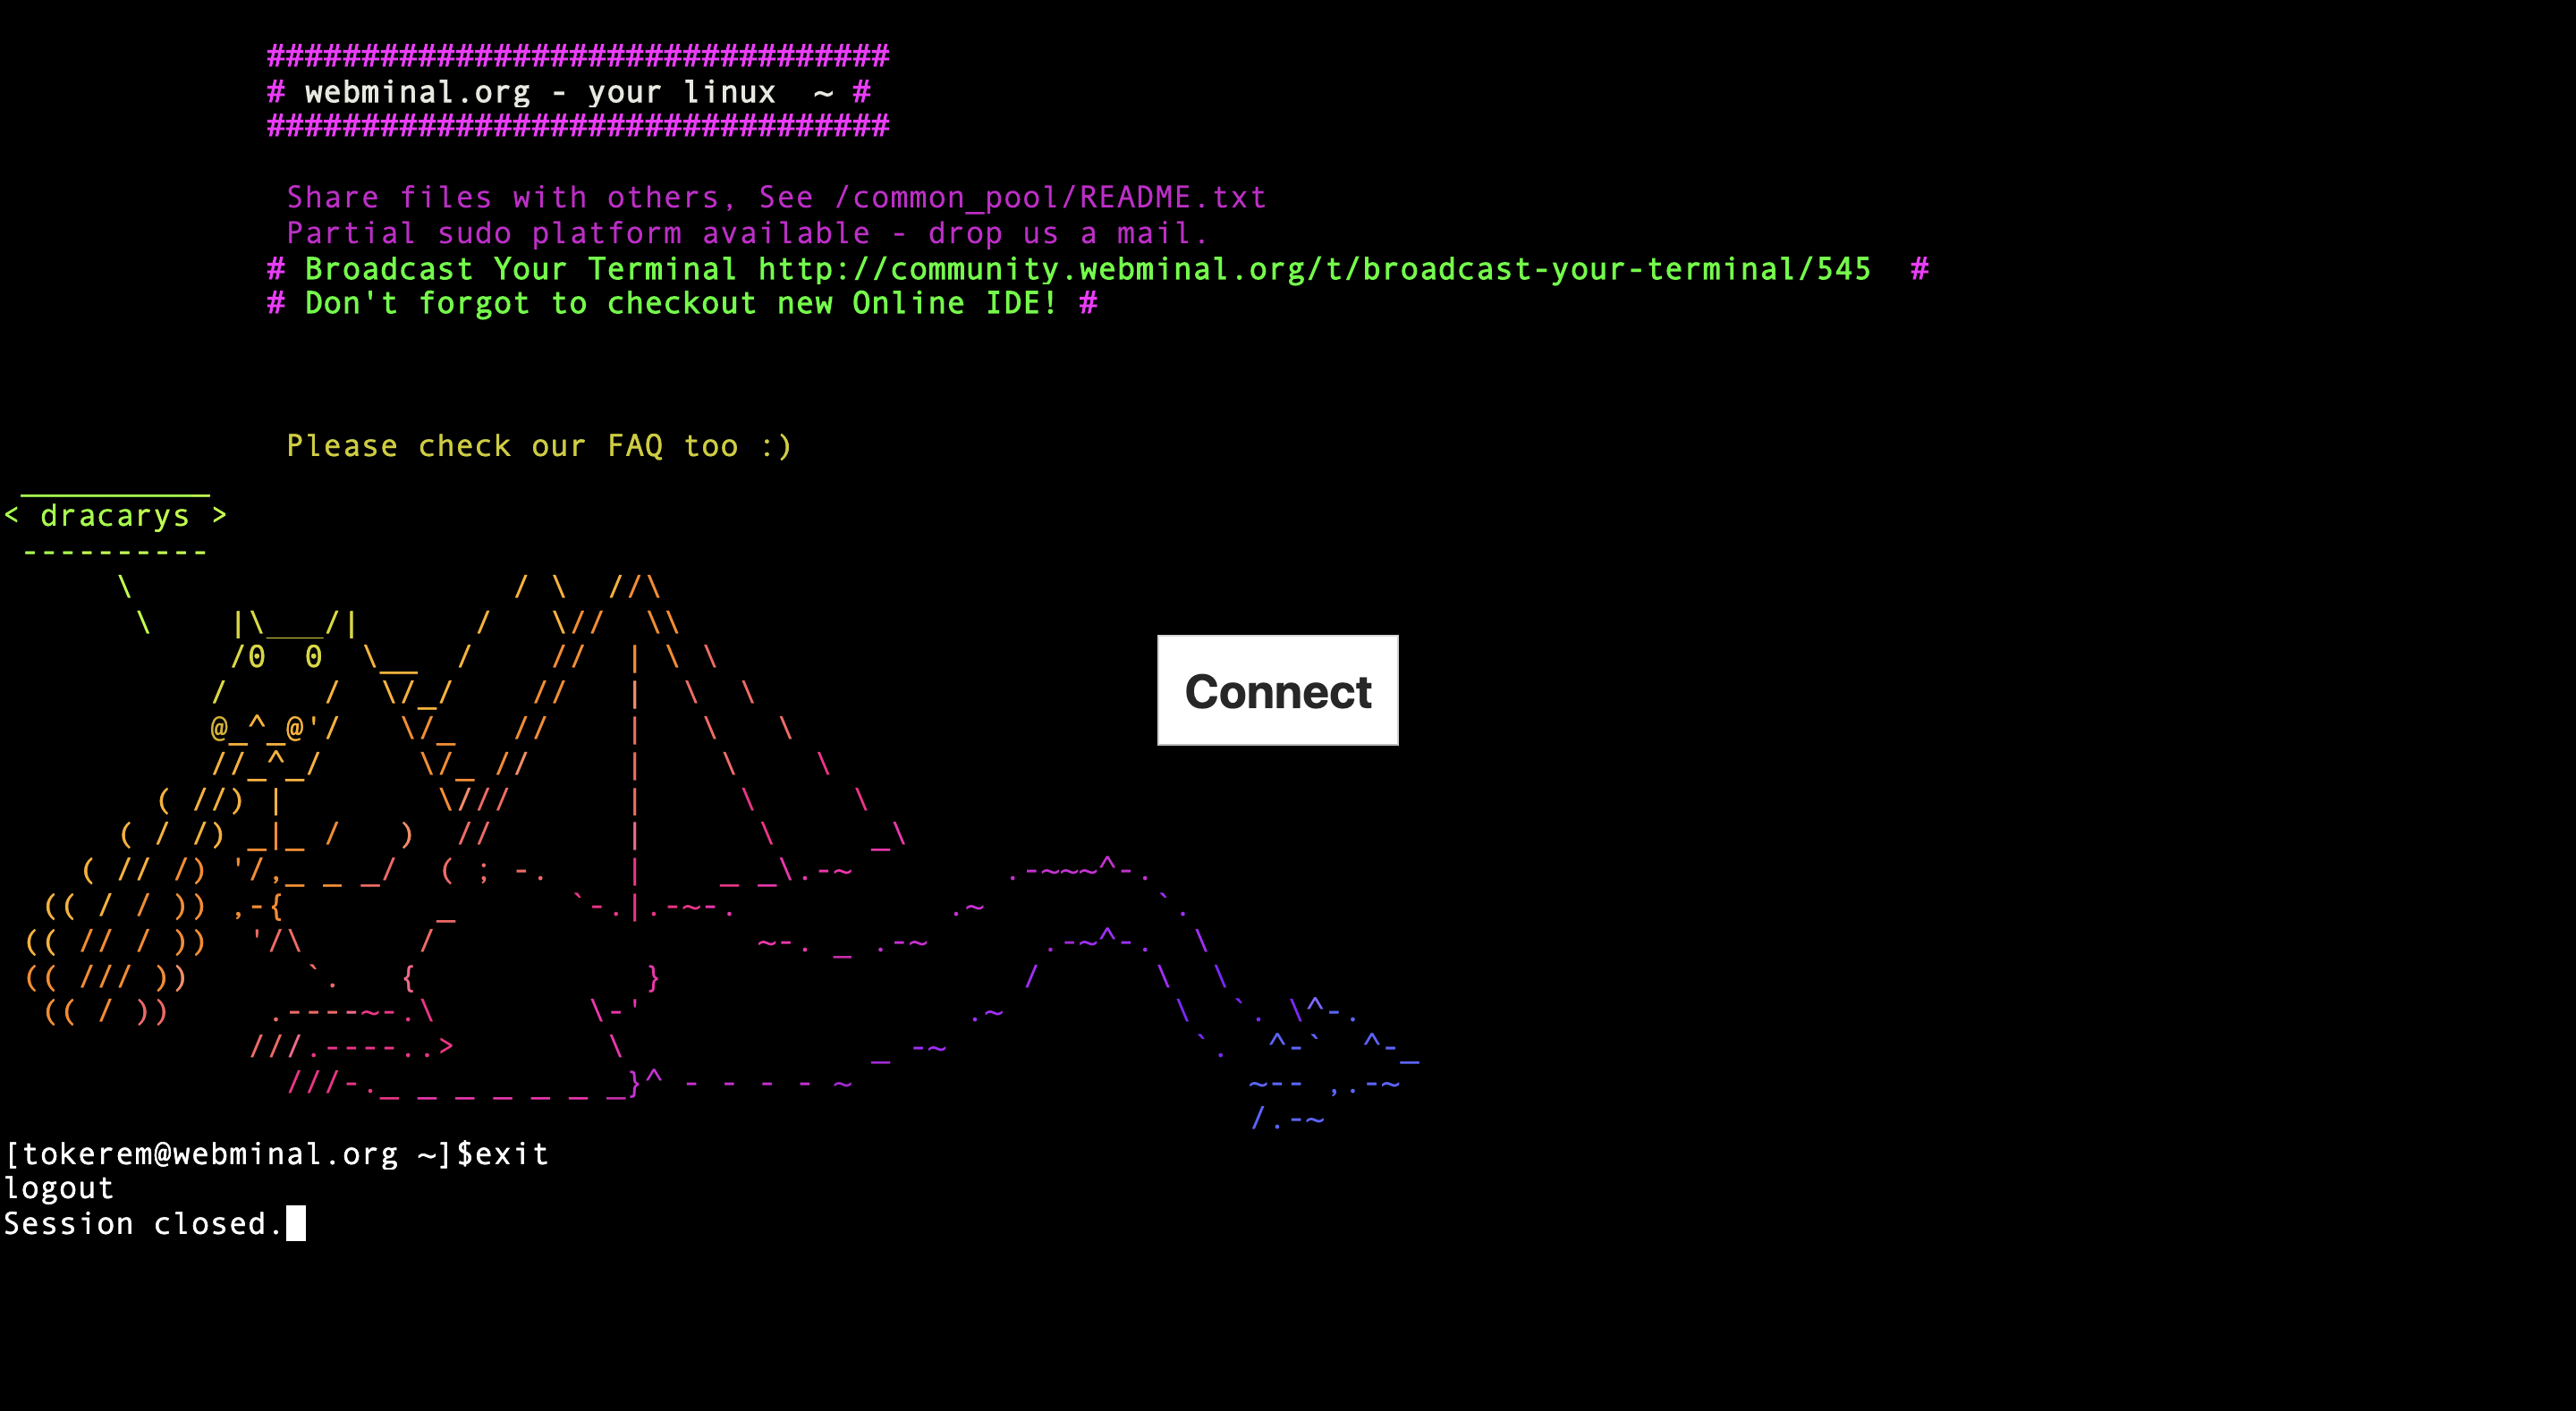
\includegraphics{exit.png}
\caption{}
\end{figure}

\end{block}

\end{frame}

\begin{frame}[fragile]{\textbf{vi Editor}}

\begin{block}{\textbf{vi Editor and Print Commands}}

\begin{itemize}
\item
  {\textbf{vi}}
\item
  {\textbf{esc}} \emph{(default mode)}
\item
  {\textbf{i}} \emph{(insert mode)}
\item
  {\textbf{:q}} \emph{(just quit)}
\item
  {\textbf{:q!}} \emph{(don't save and quit)}
\item
  {\textbf{:qw}} \emph{(write/save and quit)}
\item
  {\textbf{grep}} and {\textbf{echo}}
\item
  {\textbf{head}} and {\textbf{tail}}
\item
  {\textbf{sed}} \emph{(stream editor)}
\end{itemize}

\end{block}

\begin{block}{\textbf{vi Editor and Print Commands - {\textbf{vi}}}}

\begin{figure}
\centering
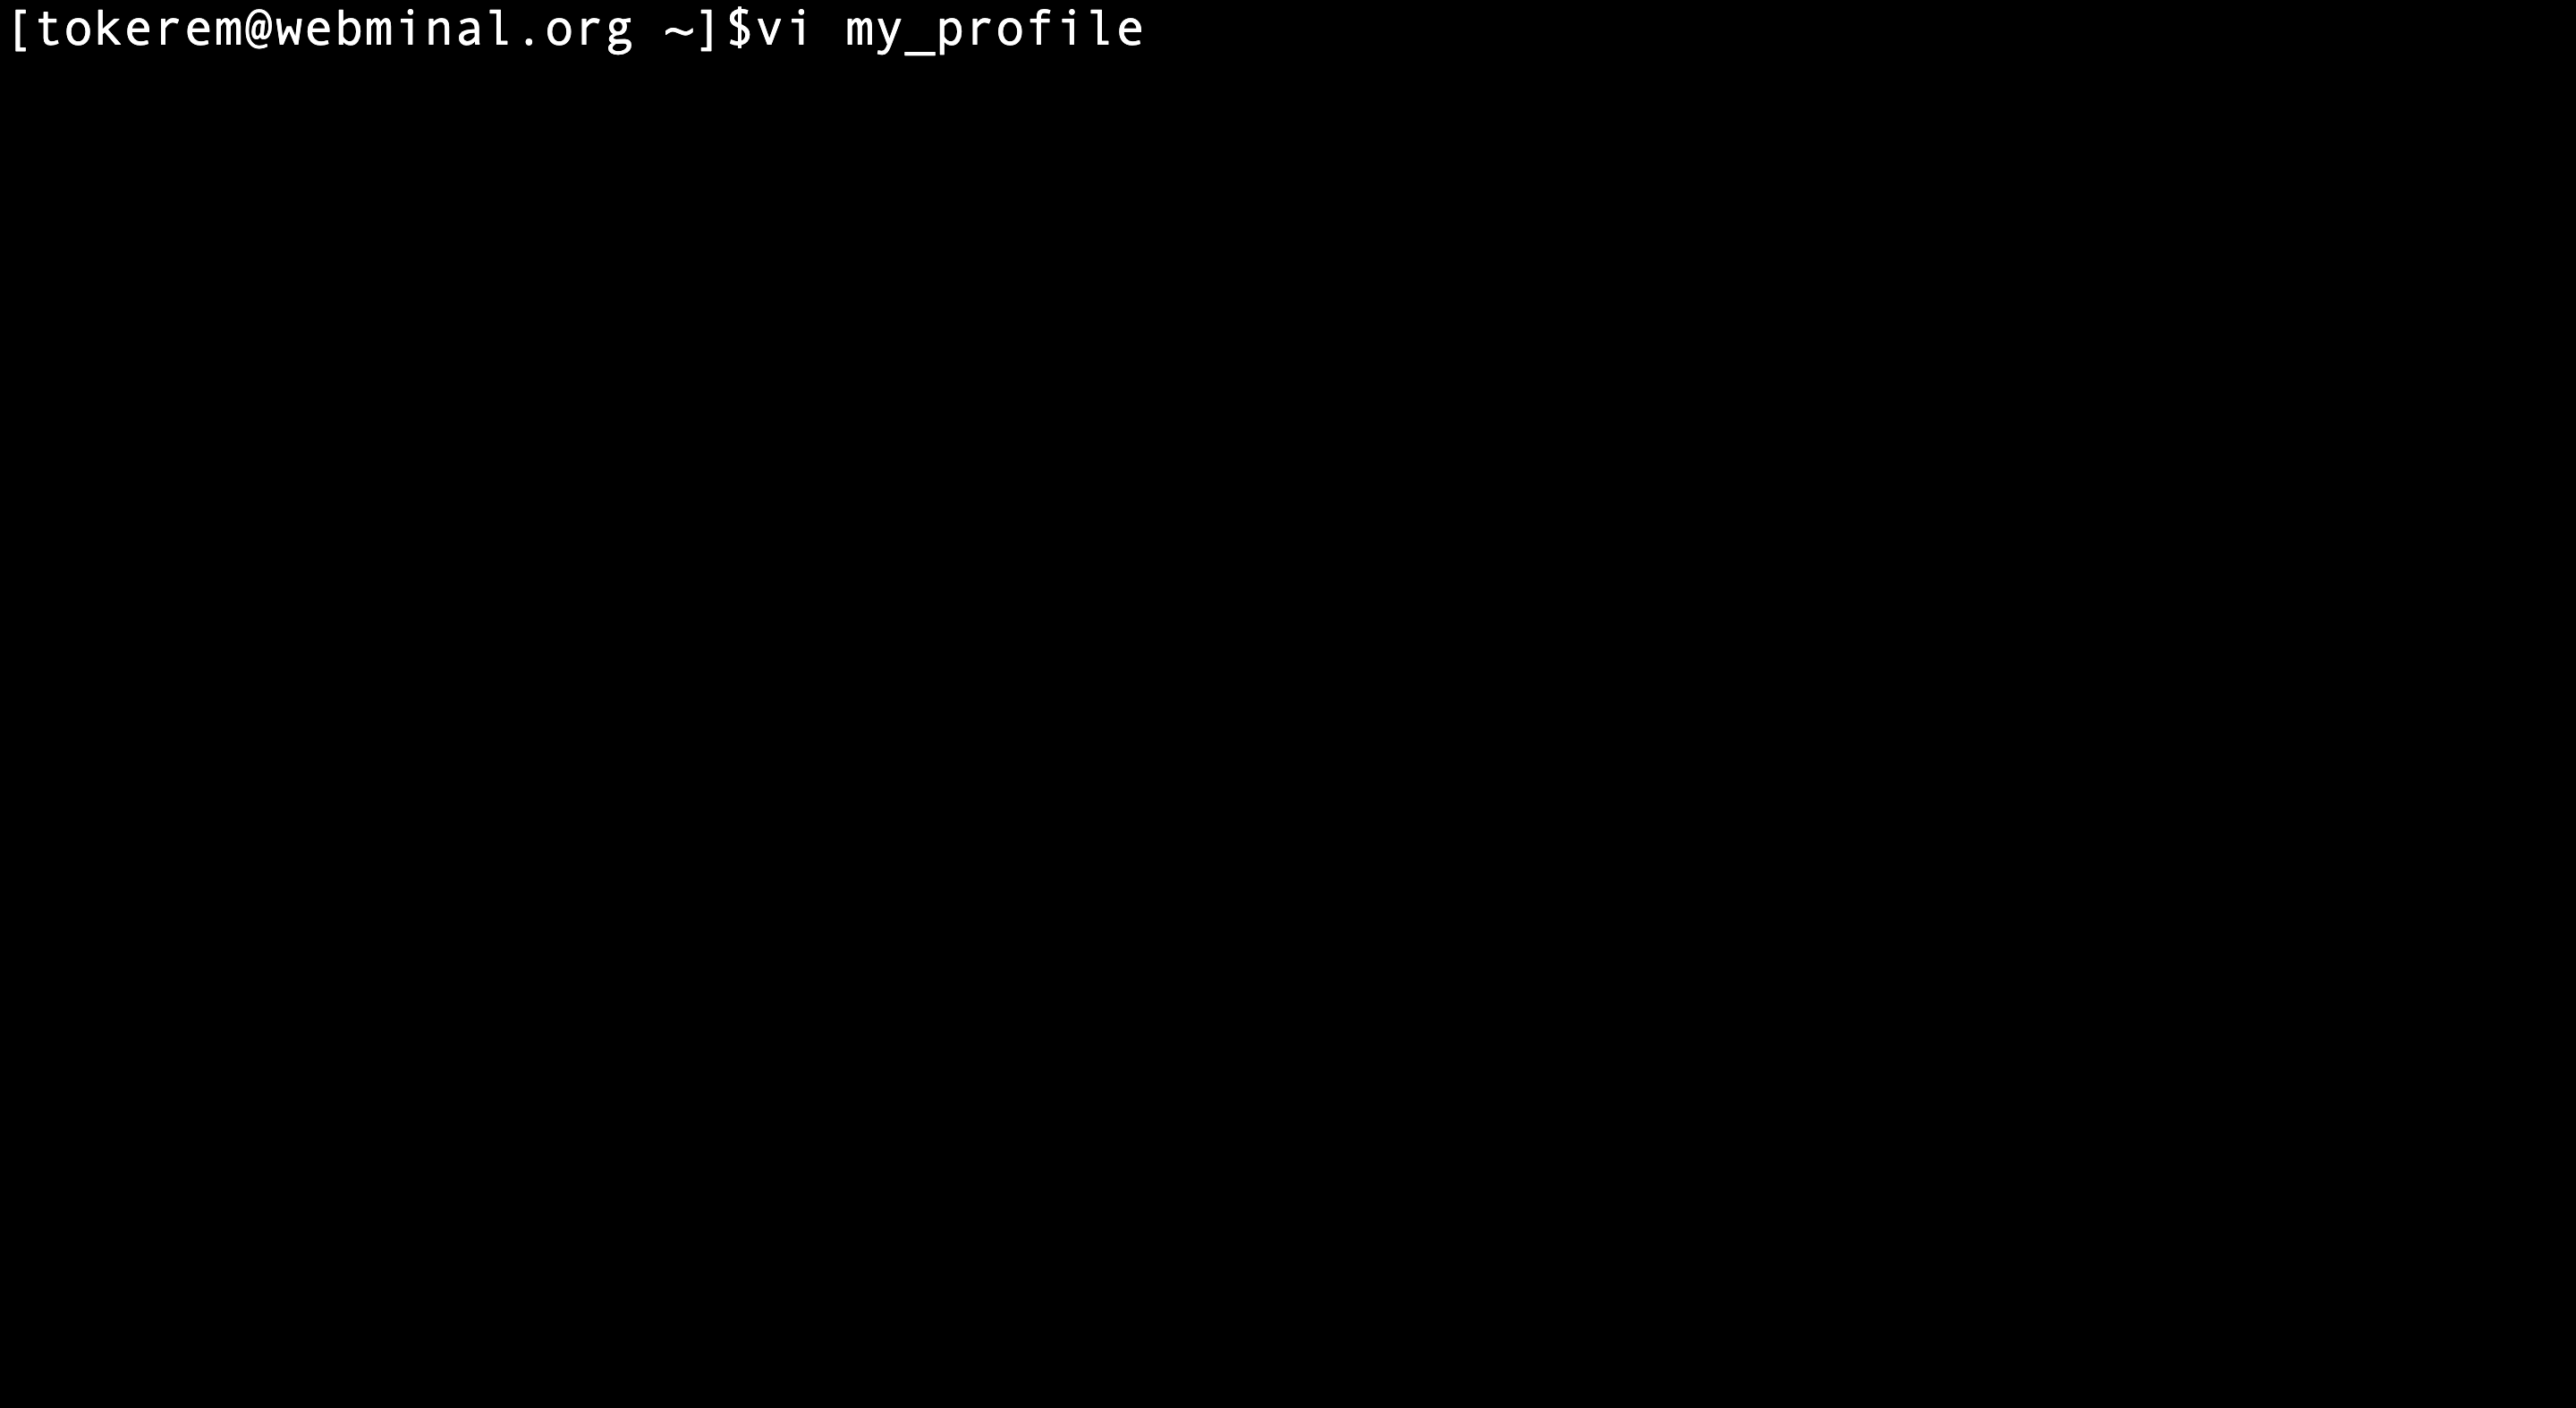
\includegraphics{vi_0.png}
\caption{}
\end{figure}

\end{block}

\begin{block}{\textbf{vi Editor and Print Commands - {\textbf{esc}}}}

\emph{(Default Mode)}

\begin{figure}
\centering
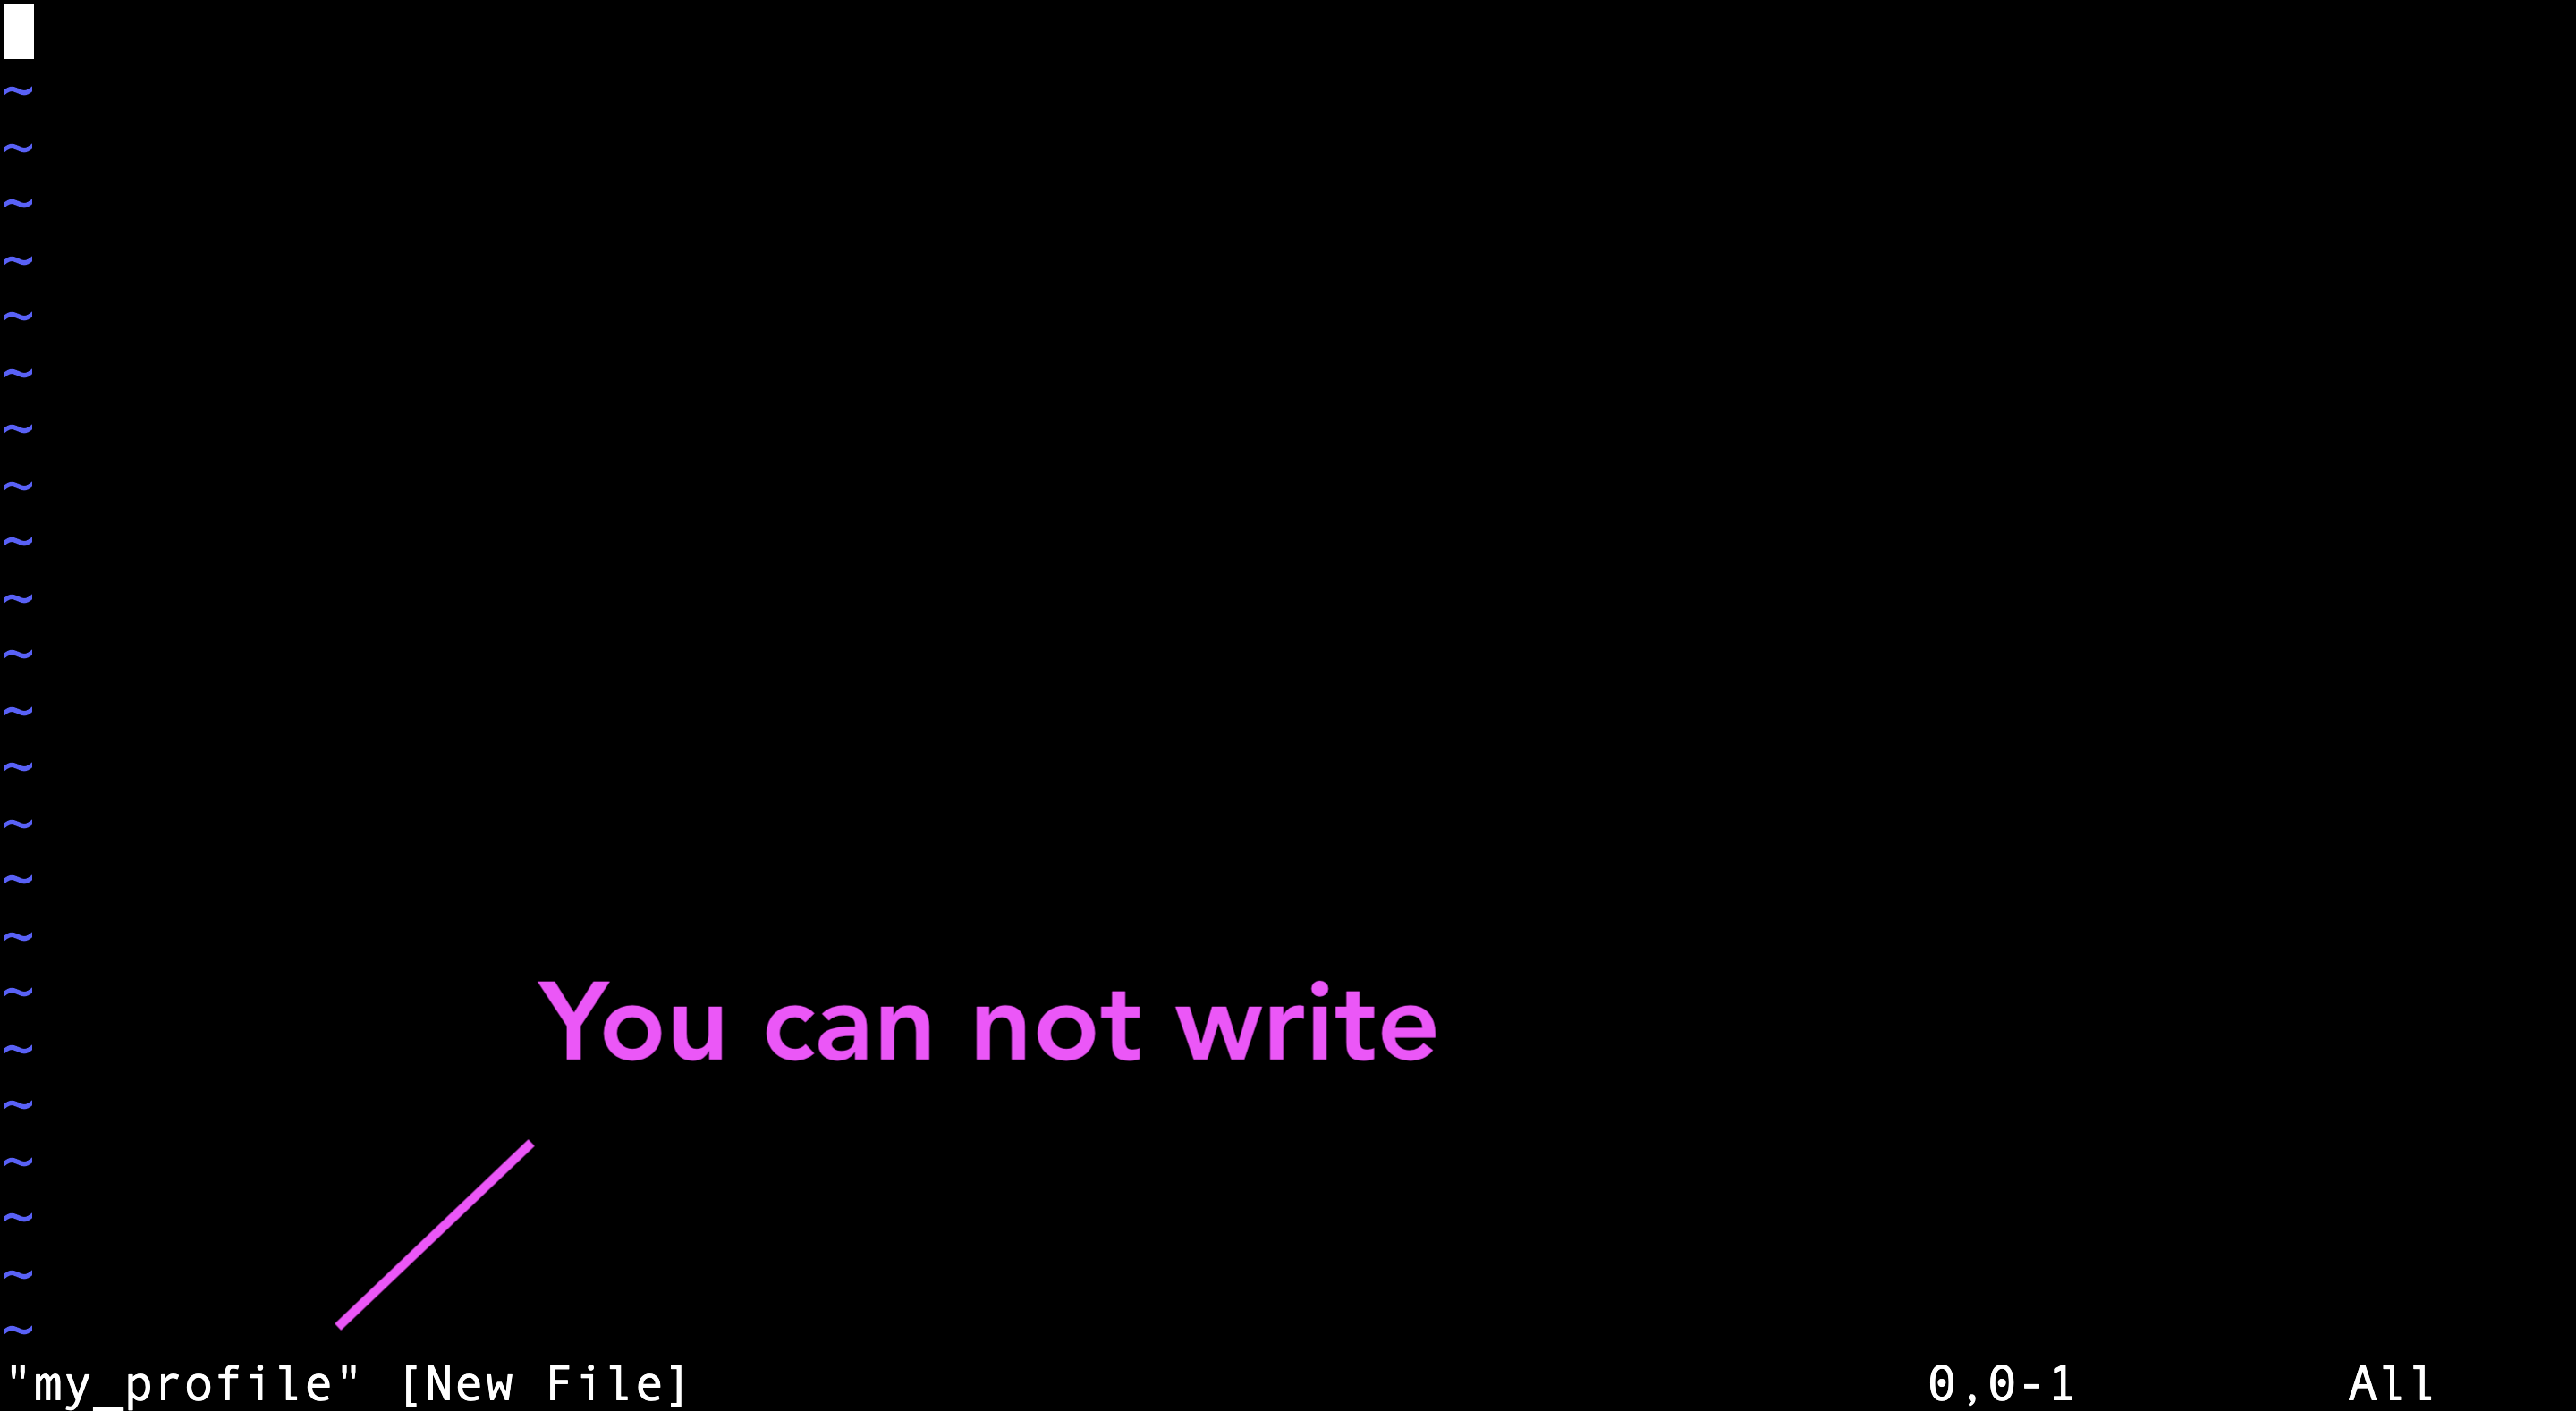
\includegraphics{vi_1.png}
\caption{}
\end{figure}

\end{block}

\begin{block}{\textbf{vi Editor and Print Commands - {\textbf{i}}}}

\emph{(Insert Mode)}

\begin{figure}
\centering
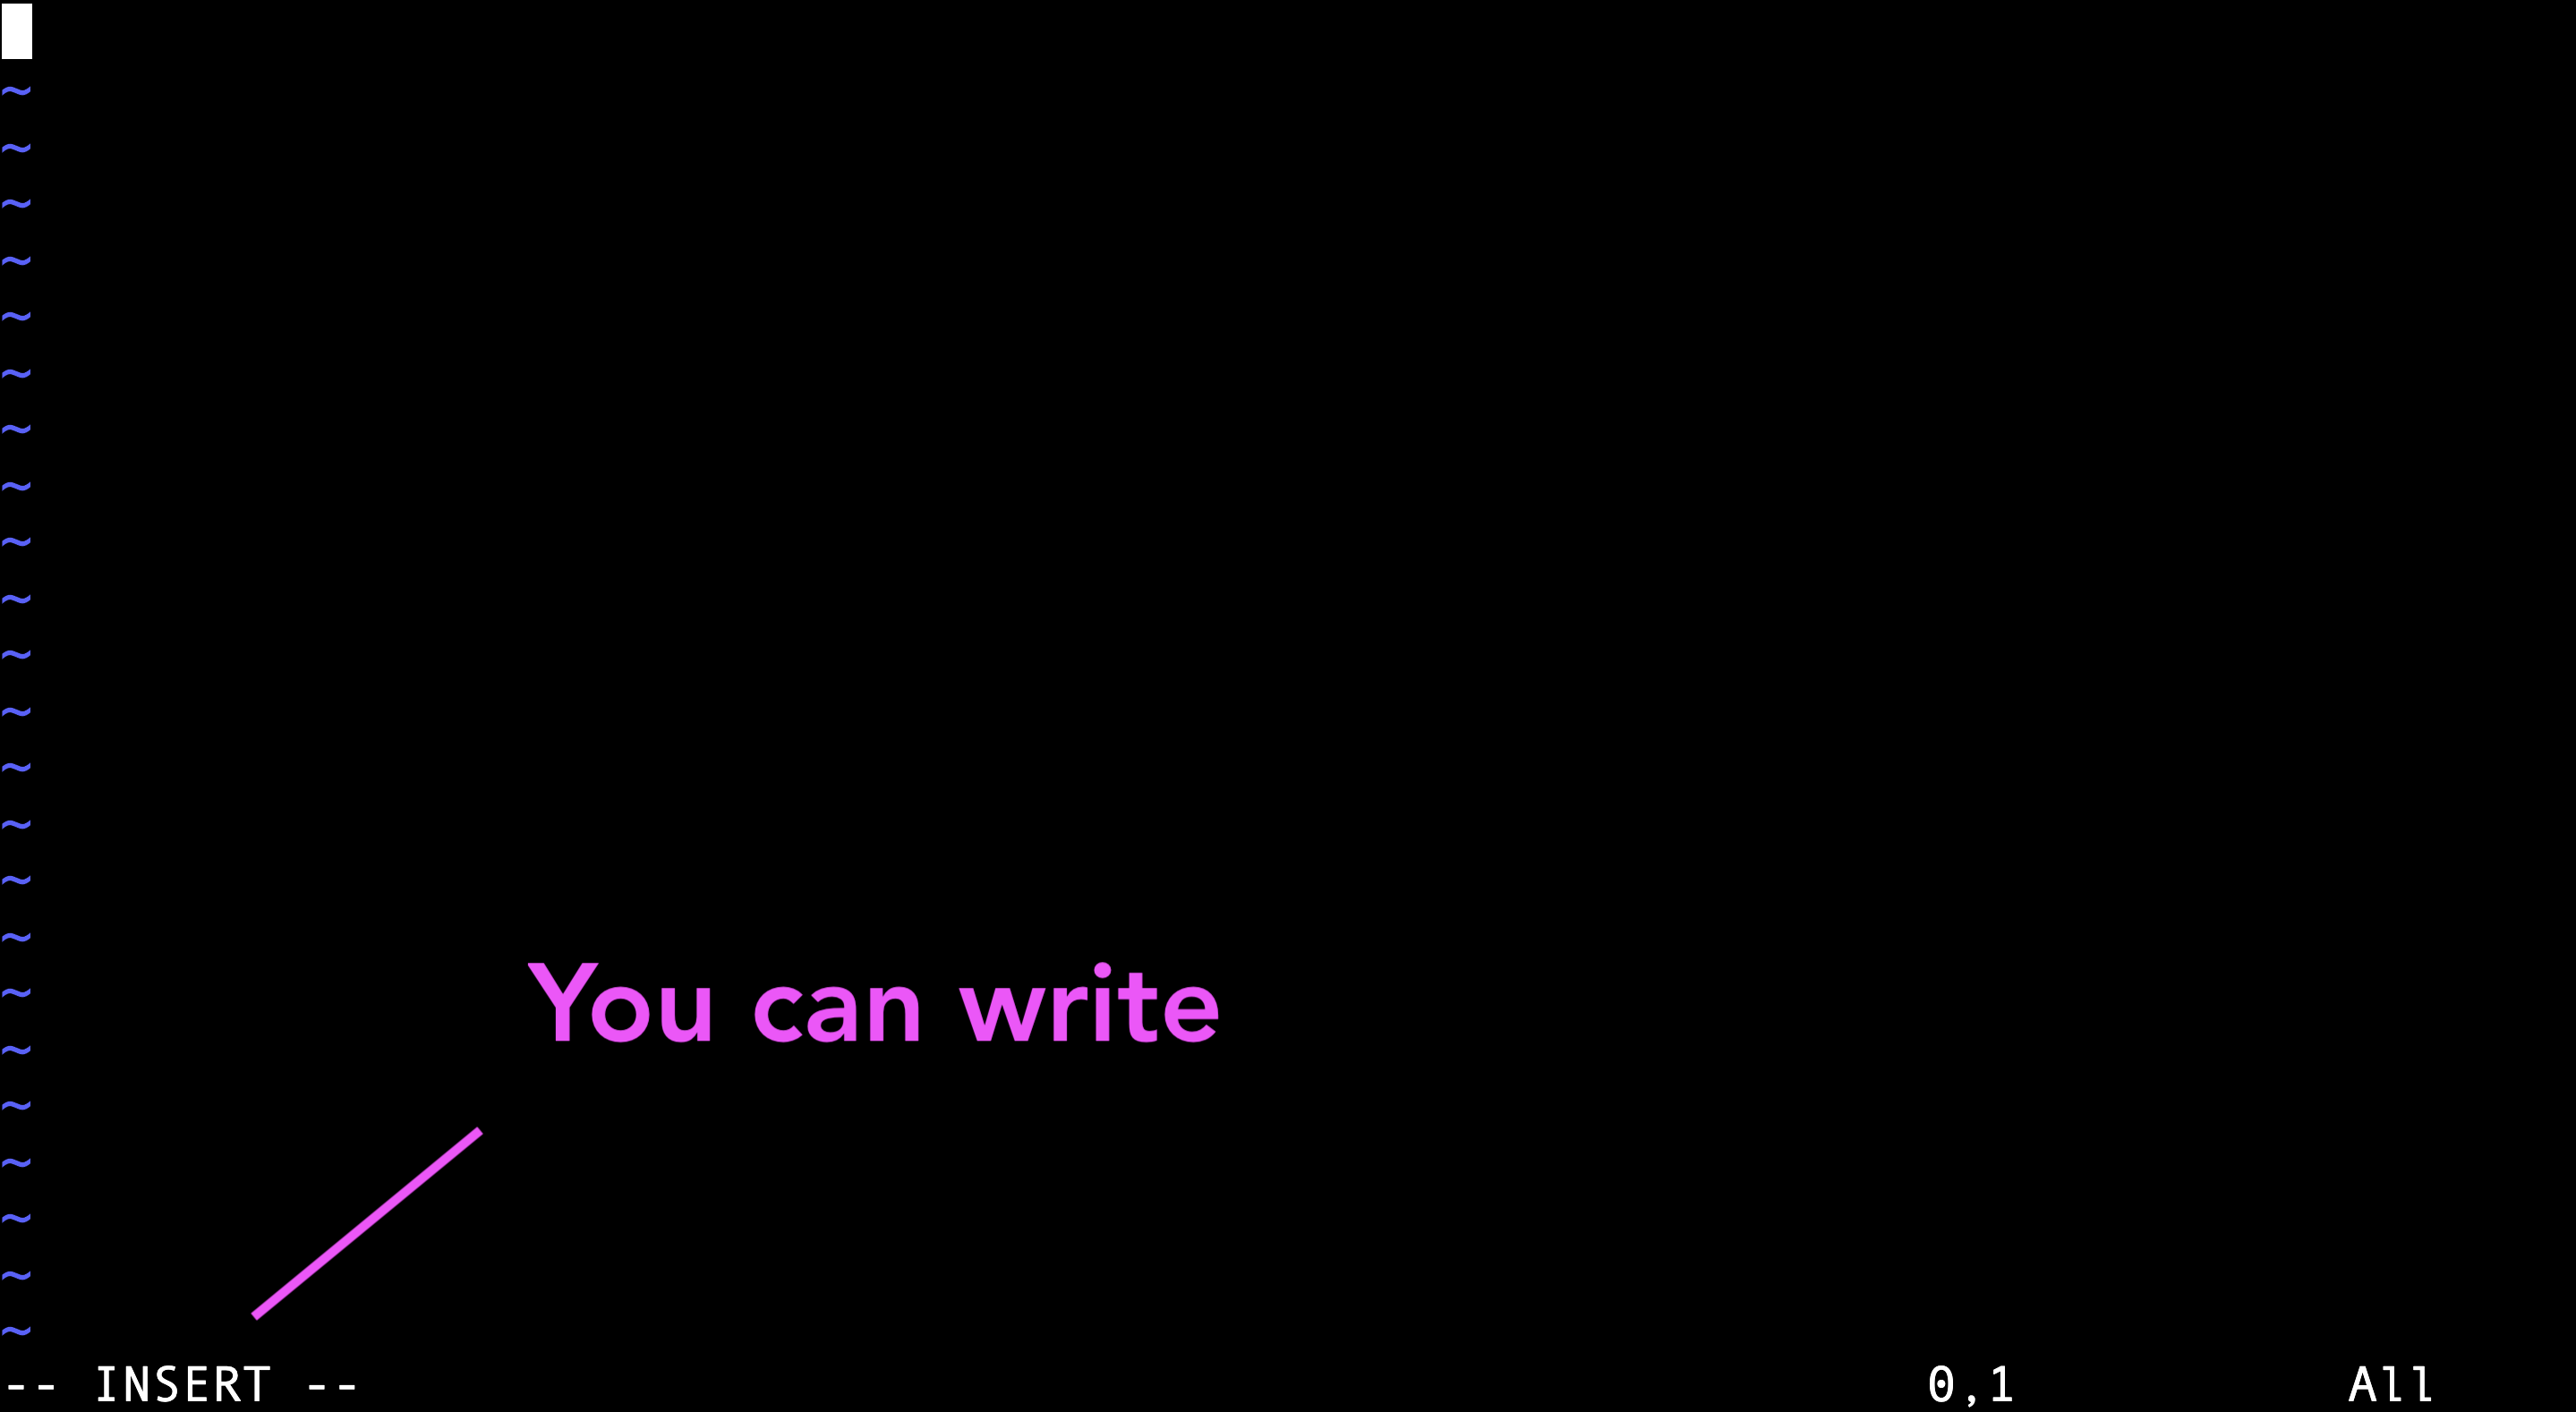
\includegraphics{vi_2.png}
\caption{}
\end{figure}

\end{block}

\begin{block}{\textbf{vi Editor and Print Commands - {\textbf{:wq}}}}

\emph{(Write/Save and Quit)}

\begin{figure}
\centering
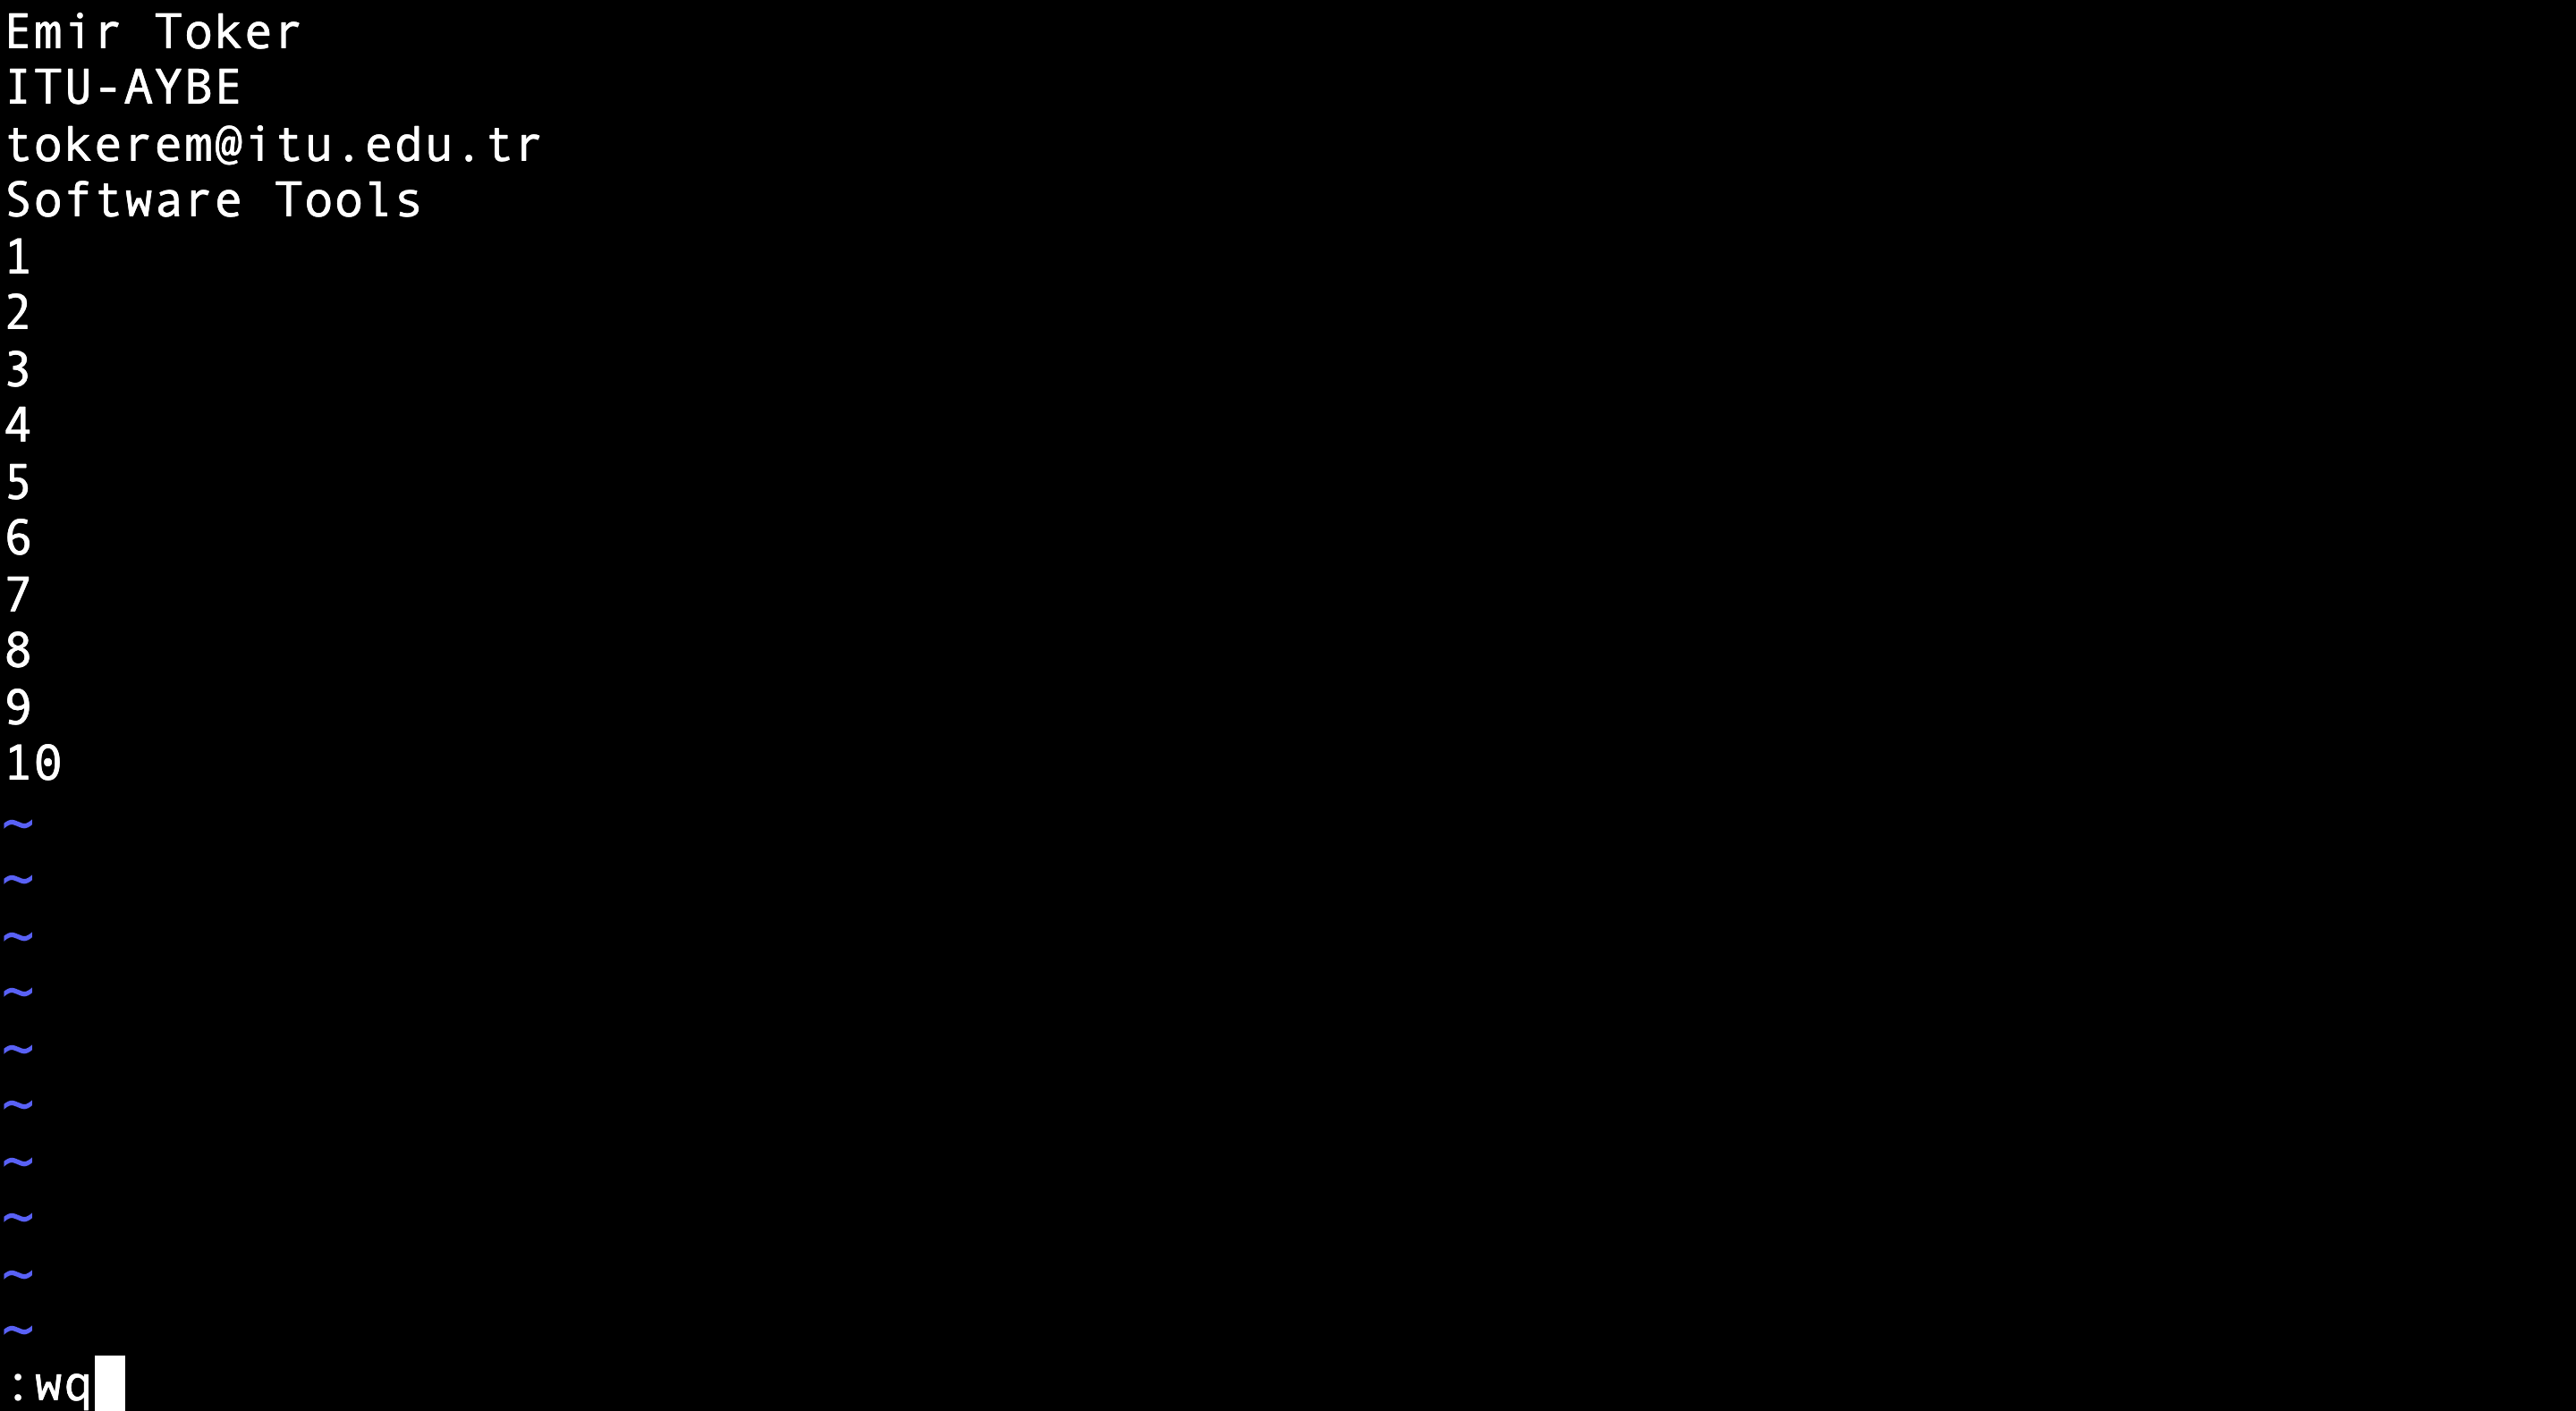
\includegraphics{vi_3.png}
\caption{}
\end{figure}

\end{block}

\begin{block}{\textbf{vi Editor and Print Commands - {\textbf{grep}} and
{\textbf{echo}}}}

\begin{verbatim}
grep my_profile
\end{verbatim}

\begin{verbatim}
grep ITU my_profile
\end{verbatim}

\begin{verbatim}
echo my_profile
\end{verbatim}

\begin{verbatim}
name=Emir
\end{verbatim}

\begin{verbatim}
echo $name
\end{verbatim}

\end{block}

\begin{block}{\textbf{vi Editor and Print Commands - {\textbf{head}} and
{\textbf{tail}}}}

\begin{verbatim}
head my_profile
\end{verbatim}

\begin{verbatim}
tail my_profile
\end{verbatim}

\end{block}

\begin{block}{vi Editor and Print Commands - {\textbf{sed}}}

\emph{(Stream Editor)}

Replacing or substituting string;

\begin{verbatim}
sed 's/ITU/ODTU/' my_profile
\end{verbatim}

\begin{verbatim}
sed '5d' my_profile 
\end{verbatim}

\end{block}

\end{frame}

\begin{frame}[fragile]{Symbols}

\begin{block}{Symbols}

\begin{itemize}
\tightlist
\item
  {\textbf{\textbar{}}} \emph{(and)}
\item
  {\textbf{\textgreater{}}} \emph{(assing)}
\item
  {\textbf{\$}} \emph{(special variable)}
\item
  {\textbf{?}} \emph{(an unknown character)}
\item
  {\texttt{*}} \emph{(an unknown sroup of characters)}
\end{itemize}

\begin{verbatim}
cat my_profile | sort
\end{verbatim}

\begin{verbatim}
ls > my_list
\end{verbatim}

\begin{verbatim}
x=3
echo $x
\end{verbatim}

\begin{verbatim}
ls my*
\end{verbatim}

\begin{verbatim}
ls ?y_list* 
\end{verbatim}

\end{block}

\end{frame}

\begin{frame}[fragile]{BONUS}

\begin{block}{Bash Script}

\begin{verbatim}
touch my_bash_script.sh
vi my_bash_script.sh
\end{verbatim}

\begin{verbatim}
x=5
y=3
echo $((x+y))
\end{verbatim}

\begin{verbatim}
bash my_bash_script.sh
\end{verbatim}

\begin{verbatim}
8
\end{verbatim}

\end{block}

\end{frame}

\begin{frame}[fragile]{Practice and Quiz}

\begin{block}{Practice}

\begin{enumerate}
\def\labelenumi{\arabic{enumi}.}
\tightlist
\item
  \textbf{Learn where you are} \emph{(Print your working directory)}
\item
  \textbf{Look at inside} \emph{(list all documents and directories)}
\item
  \textbf{Create a new folder} \emph{(make a
  directory,\texttt{\textless{}my\_new\_dir\textgreater{}})}
\item
  \textbf{Go to the \texttt{\textless{}my\_new\_dir\textgreater{}}}
  \emph{(change your directory)}
\item
  \textbf{Create a new file} \emph{(touch it, file name :
  \texttt{\textless{}my\_new\_file\textgreater{}})}
\item
  \textbf{Open this new file and write your name} \emph{(vi-insert
  mode)}
\item
  \textbf{Save your work and close the file} \emph{(write + quit)}
\item
  \textbf{Print your name on the screen} \emph{(grep, tail, head, cat)}
\item
  \textbf{Put \texttt{\textless{}my\_new\_file\textgreater{}} at the
  parent directory} \emph{(move it)}
\item
  \textbf{Go to parent directory} (change directory with two dots)
\item
  \textbf{Create a copy, name;
  \texttt{\textless{}my\_new\_file\_2\textgreater{}}}
\item
  \textbf{Remove your first folder
  \texttt{\textless{}my\_new\_dir\textgreater{}}}
\item
  \textbf{List all documents and directories}
\end{enumerate}

\end{block}

\begin{block}{Quiz}

\begin{figure}
\centering

\includegraphics{linux_logo.png}
\caption{}
\end{figure}

Introduction to Gnu/Linux

\href{https://create.kahoot.it/details/1932babe-f920-47bc-9216-802e5c3d294d}{LINK}

\end{block}

\end{frame}

\begin{frame}[fragile]{\textbf{Python and Jupyter}}

\begin{block}{\textbf{What is the Python}}

\begin{itemize}
\tightlist
\item
  Python is a programming language.
\item
  Created by Guido van Rossum and first released in 1991.
\item
  Python 2.0, released 2000, Python 3.0, released 2008.
\item
  Python 2.7, the last release in the 2.x series, was extended to 2020.
\end{itemize}

\begin{figure}
\centering

\includegraphics{python.jpg}
\caption{}
\end{figure}

\end{block}

\begin{block}{\textbf{Python in Terminal}}

\href{https://www.webminal.org/terminal/}{webminal.org}

\begin{figure}
\centering
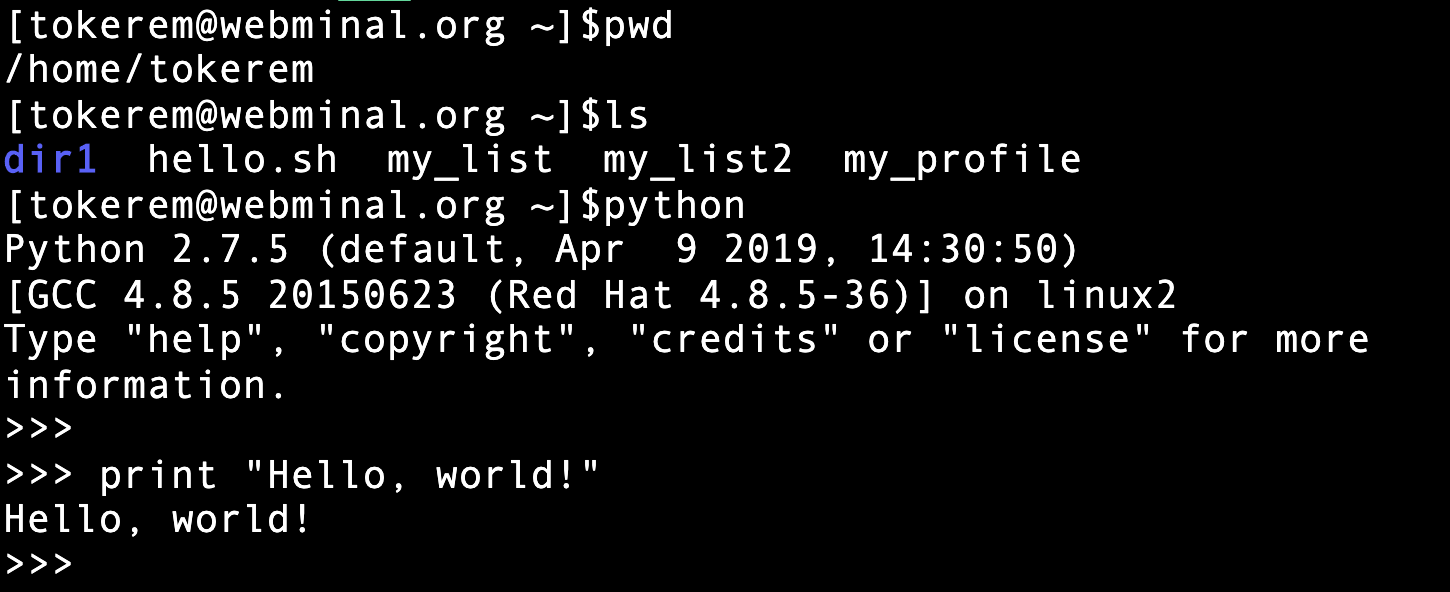
\includegraphics{python_term.png}
\caption{}
\end{figure}

GCC : GNU Compiler Collection

\end{block}

\begin{block}{\textbf{What is the Anaconda/Jupyter}}

\begin{figure}
\centering
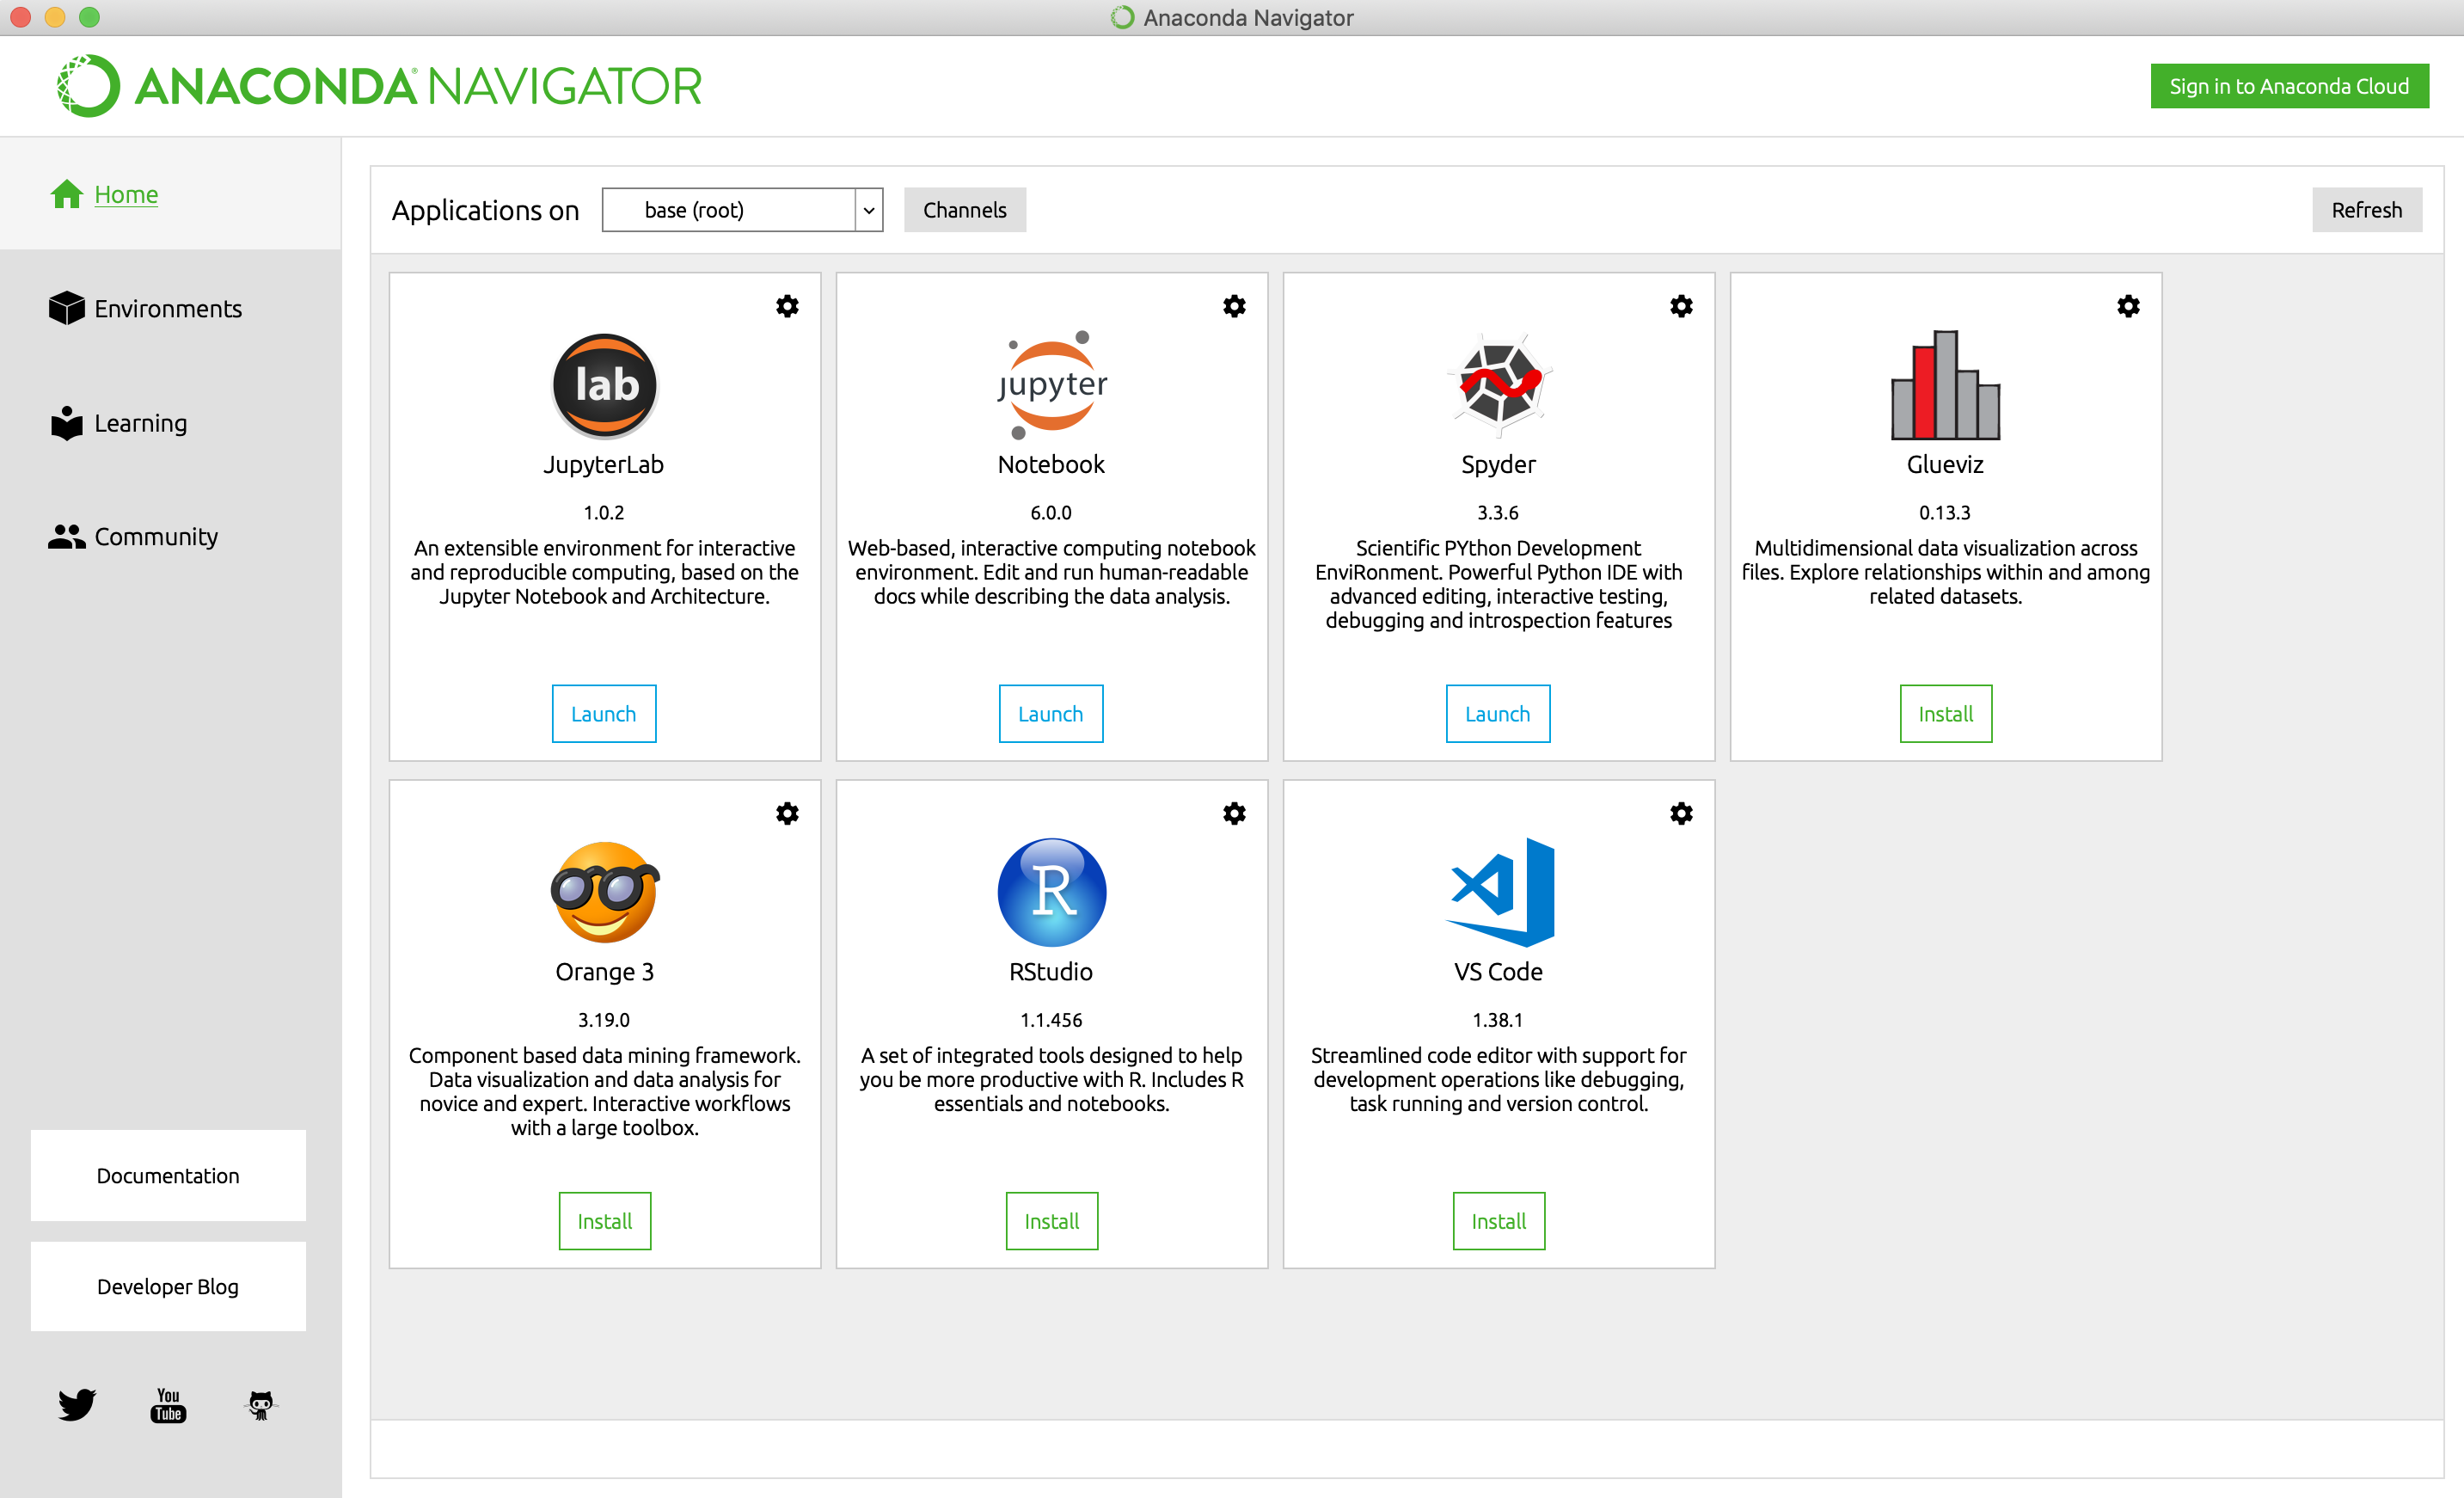
\includegraphics{conda.png}
\caption{}
\end{figure}

\end{block}

\begin{block}{\textbf{Python in Anaconda/Jupyter}}

\begin{verbatim}
jupyter notebook
\end{verbatim}

\begin{figure}
\centering
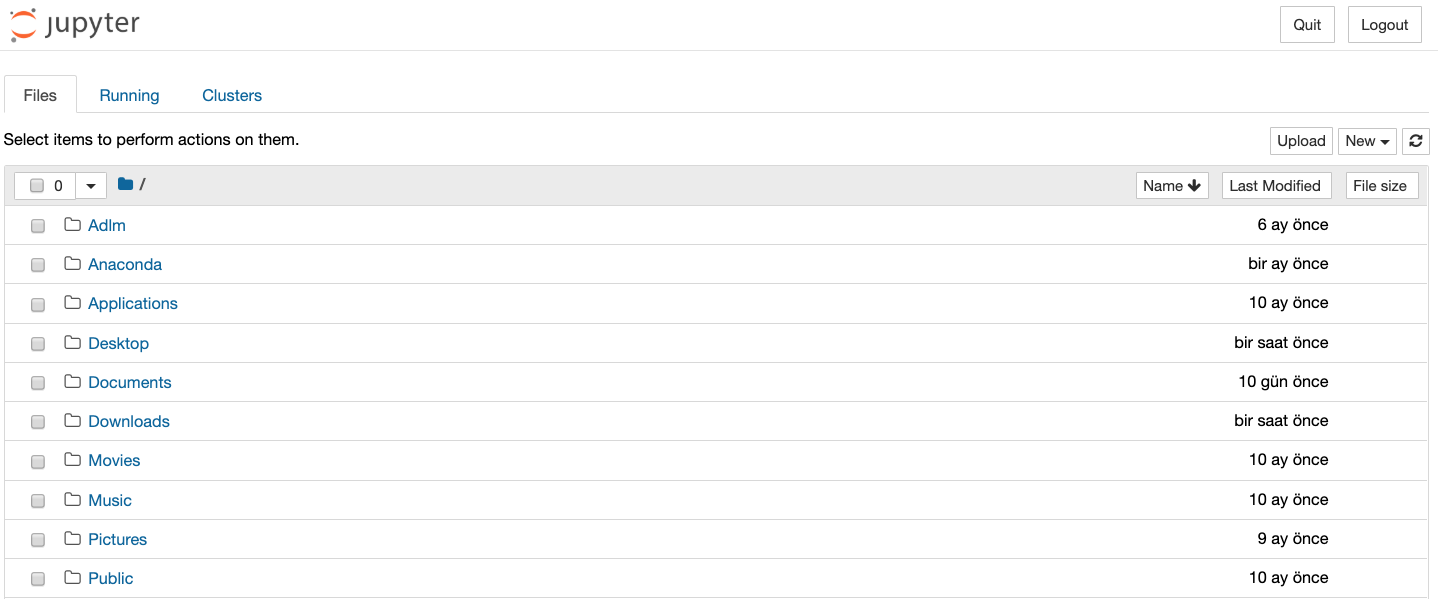
\includegraphics{jupyter_notebook.png}
\caption{}
\end{figure}

\end{block}

\end{frame}

\begin{frame}{\textbf{Next Week}}

\begin{itemize}
\item
  Data Fortmats, Sources and Download
\item
  NCL, nco, cdo
\end{itemize}

\end{frame}

\end{document}
